% 第 3 章 矩阵 (Matrizen)
\chapter{矩阵}\index{juzhen@矩阵(Matrix)}

\section*{预备说明}

迄今为止, 我们主要研究了向量空间与线性映射的基本性质以及与此相关的各种构造.现在我们要进一步强调计算的观点, 并在此章中说明, 如何有效地计算求解线性代数中具体给出的问题.这里的中心是矩阵与所谓的高斯(Gauß)消元法, 特别是用于求解线性方程组的那一版本.

作为例子, 我们从如下的几何情形出发:

\begin{center}
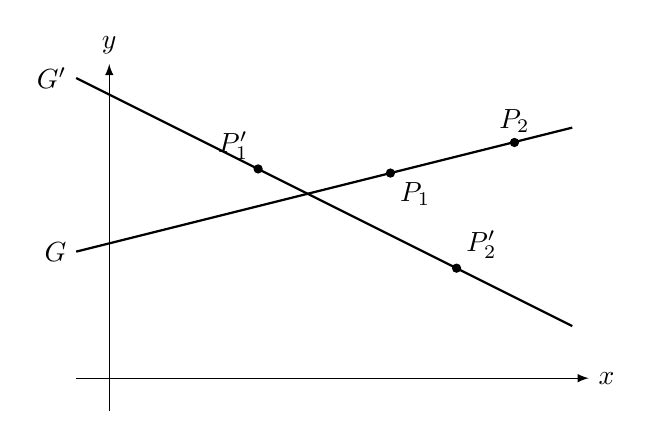
\begin{tikzpicture}[>=latex, scale=1.05]
  \draw[->] (-0.4,0) -- (5.8,0) node[right]{$x$};
  \draw[->] (0,-0.4) -- (0,3.8) node[above]{$y$};
  
  % 直线 G' (负斜率)
  \draw[thick] (-0.4,3.63) -- (5.6,0.63);
  \node[left] at (-0.4,3.63) {$G'$};
  \coordinate (P1p) at (1.8,2.53);
  \coordinate (P2p) at (4.2,1.33);
  \fill (P1p) circle (1.6pt) node[above left]{$P_1'$};
  \fill (P2p) circle (1.6pt) node[above right]{$P_2'$};
  
  % 直线 G (正斜率)
  \draw[thick] (-0.4,1.53) -- (5.6,3.03);
  \node[left] at (-0.4,1.53) {$G$};
  \coordinate (P1) at (3.4,2.48);
  \coordinate (P2) at (4.9,2.85);
  \fill (P1) circle (1.6pt) node[below right]{$P_1$};
  \fill (P2) circle (1.6pt) node[above]{$P_2$};
\end{tikzpicture}
\end{center}

给定两条直线 $G, G' \subset \mathbb{R}^2$, 其中 $G$ 由(不同的)两点 $P_1, P_2 \in \mathbb{R}^2$ 确定, 相应地 $G'$ 由(不同的)两点 $P_1', P_2' \in \mathbb{R}^2$ 确定.于是要根据 $P_1, P_2, P_1', P_2'$ 研究 $G$ 与 $G'$ 是否具有交点, 即公共点, 若有, 又如何从点 $P_1, P_2, P_1', P_2'$ 计算出这些交点.正如我们在第 1 章的预备说明中已经看到的, $G$ 与 $G'$ 具有参数表示

\[
G = \left\{P_1 + t(P_2 - P_1);\; t \in \mathbb{R}\right\}, \qquad
G' = \left\{P_1' + t'(P_2' - P_1');\; t' \in \mathbb{R}\right\},
\]

而交点 $S \in G \cap G'$ 显然刻画为: 存在参数 $t, t' \in \mathbb{R}$ 使得

\[
P_1 + t(P_2 - P_1) = S = P_1' + t'(P_2' - P_1')\text{.}
\]

换言之, 为求 $G$ 与 $G'$ 的交点, 我们必须确定满足方程

\begin{equation}
t(P_2 - P_1) + t'(P_1' - P_2') = P_1' - P_1 \tag{$*$}
\end{equation}

的一切数对 $(t, t') \in \mathbb{R}^2$; 或者, 在分量记号

\[
P_2 - P_1 = (\alpha_{11}, \alpha_{21}), \qquad
P_1' - P_2' = (\alpha_{12}, \alpha_{22}), \qquad
P_1' - P_1 = (\beta_1, \beta_2)
\]

之下, 即满足方程组

\begin{equation}
\begin{array}{c}
t\alpha_{11} + t'\alpha_{12} = \beta_1, \\
t\alpha_{21} + t'\alpha_{22} = \beta_2
\end{array} \tag{$**$}
\end{equation}

的一切数对.于是要解一个由 $2$ 个方程组成的方程组, 其中含两个未知量 $t, t'$ 及给定的常数 $\alpha_{ij}, \beta_i \in \mathbb{R}$.这里涉及的是一个线性方程组, 其含义是: 未知量 $t, t'$ 彼此分离, 且至多以一次幂出现.

为解方程 $(*)$, 我们首先假设两个向量 $P_2 - P_1$ 与 $P_1' - P_2'$ 线性相关, 此时每个向量都是另一个的标量倍; 几何上这意味着 $G$ 与 $G'$ 平行.于是 $P_1' - P_2'$ 是 $P_2 - P_1$ 的一个标量倍, 比如说 $P_1' - P_2' = \gamma(P_2 - P_1)$, 从而可以把方程 $(*)$ 改写为

\[
P_1' = P_1 + (t + \gamma t')(P_2 - P_1)\text{.}
\]

因此解 $t, t'$ 的存在性等价于 $P_1' \in G$, 而这已经蕴含 $G = G'$.于是只可能发生下列互相排斥的情形:

\begin{enumerate}
\item $P_2 - P_1$ 与 $P_1' - P_2'$ 线性相关, $G = G'$;
\item $P_2 - P_1$ 与 $P_1' - P_2'$ 线性相关, $G \neq G'$; 此时 $G \cap G' = \varnothing$;
\item $P_2 - P_1$ 与 $P_1' - P_2'$ 线性无关; 此时 $G$ 与 $G'$ 恰好有一个交点(这是直观明显的), 我们随即就要计算它.
\end{enumerate}

现在我们按情形 3 假设向量 $P_2 - P_1 = (\alpha_{11}, \alpha_{21})$ 与 $P_1' - P_2' = (\alpha_{12}, \alpha_{22})$ 线性无关.特别有 $P_2 - P_1 \neq 0$, 不妨设 $\alpha_{11} \neq 0$.于是我们可以在等价的意义下变换方程组 $(**)$, 即把第一方程的 $\frac{\alpha_{21}}{\alpha_{11}}$ 倍从第二方程中减去, 从而在第二方程中"消去"未知量 $t$:

\[
\begin{array}{r l}
t\alpha_{11} + t'\alpha_{12} &= \beta_1, \\
t'\left(\alpha_{22} - \frac{\alpha_{21}}{\alpha_{11}}\alpha_{12}\right) &= \beta_2 - \frac{\alpha_{21}}{\alpha_{11}}\beta_1\text{.}
\end{array}
\]

但此时 $\alpha_{22} - \frac{\alpha_{21}}{\alpha_{11}}\alpha_{12} \neq 0$, 因为否则将得到

\[
\alpha_{12} = \frac{\alpha_{12}}{\alpha_{11}}\alpha_{11}, \qquad
\alpha_{22} = \frac{\alpha_{12}}{\alpha_{11}}\alpha_{21},
\]

从而 $P_1' - P_2'$ 线性依赖于 $P_2 - P_1$, 这与我们的假设矛盾.于是可以把第二方程继续等价地变换为

\[
t' = \frac{\beta_2 - \frac{\alpha_{21}}{\alpha_{11}}\beta_1}{\alpha_{22} - \frac{\alpha_{21}}{\alpha_{11}}\alpha_{12}}
= \frac{\alpha_{11}\beta_2 - \alpha_{21}\beta_1}{\alpha_{11}\alpha_{22} - \alpha_{21}\alpha_{12}},
\]

并由第一方程得到

\[
t = \frac{1}{\alpha_{11}}\left(\beta_1 - \alpha_{12}\frac{\alpha_{11}\beta_2 - \alpha_{21}\beta_1}{\alpha_{11}\alpha_{22} - \alpha_{21}\alpha_{12}}\right)
= \frac{\beta_1\alpha_{22} - \beta_2\alpha_{12}}{\alpha_{11}\alpha_{22} - \alpha_{21}\alpha_{12}}\text{.}
\]

这里我们是在 $\alpha_{11} \neq 0$ 的假设下对方程作等价变换的, 因此 $t, t'$ 也确实是 $(*)$ 的解.现在还剩下 $\alpha_{11} = 0$ 的情形需要考察.此时必有 $\alpha_{21} \neq 0$, 我们可以在此假设下作相应的计算.关于 $t, t'$ 的结果可以形式上从上面的结果推得: 只需在向量 $(\alpha_{11}, \alpha_{21}), (\alpha_{12}, \alpha_{22}), (\beta_1, \beta_2)$ 中分别交换分量的次序, 这相当于交换方程组 $(**)$ 的两个方程.由于如人们容易看出的, 上面的结果在这种交换下并不改变, 于是得到在非平行直线 $G, G'$ 的情形下, 方程 $(*)$ 亦即线性方程组 $(**)$ 的解为

\[
t = \frac{\beta_1\alpha_{22} - \beta_2\alpha_{12}}{\alpha_{11}\alpha_{22} - \alpha_{21}\alpha_{12}}, \qquad
t' = \frac{\alpha_{11}\beta_2 - \alpha_{21}\beta_1}{\alpha_{11}\alpha_{22} - \alpha_{21}\alpha_{12}}\text{.}
\]

特别地, $G \cap G'$ 恰由一个交点组成, 它分别作为 $G$ 与 $G'$ 的点由

\[
S = P_1 + \frac{\beta_1\alpha_{22} - \beta_2\alpha_{12}}{\alpha_{11}\alpha_{22} - \alpha_{21}\alpha_{12}}(P_2 - P_1)
= P_1' + \frac{\alpha_{11}\beta_2 - \alpha_{21}\beta_1}{\alpha_{11}\alpha_{22} - \alpha_{21}\alpha_{12}}(P_2' - P_1')
\]

计算出来.

类似地, 求 $\mathbb{R}^3$ 中两个平面的交, 或更一般地求 $K^n$ 中两个仿射子空间的交, 都归结为线性方程组.前一种情形例如是含 $4$ 个未知量的 $3$ 个方程组成的方程组, 其中在一般情况下有一个未知量可自由选取, 从而交被参数化为一条直线.后一种情形要考虑含 $r + s$ 个未知量的 $n$ 个方程组成的方程组, 其中 $r$ 与 $s$ 是所考察的 $K^n$ 中仿射子空间的维数.

甚至关于向量空间中向量的直接问题也可能导致线性方程组.例如在域 $K$ 上考虑向量 $a_i = (\alpha_{1i}, \ldots, \alpha_{ni}) \in K^n$, $i = 1, \ldots, r$, 检验它们是否线性相关.于是我们必须判断是否存在不全为零的元素 $t_1, \ldots, t_r \in K$ 使得

\[
t_1 a_1 + \cdots + t_r a_r = 0
\]

成立; 或者, 转到各个分量, 线性方程组

\[
\begin{array}{c}
t_1\alpha_{11} + \cdots + t_r\alpha_{1r} = 0, \\
t_1\alpha_{21} + \cdots + t_r\alpha_{2r} = 0, \\
\cdots \\
t_1\alpha_{n1} + \cdots + t_r\alpha_{nr} = 0
\end{array}
\]

是否具有非平凡解 $t_1, \ldots, t_r \in K$.或者我们考虑把标准基(由单位向量 $e_1, \ldots, e_r \in K^r$ 组成)映到向量 $a_1, \ldots, a_r \in K^n$ 的线性映射 $f \colon K^r \longrightarrow K^n$, 然后问: 给定的向量 $b = (\beta_1, \ldots, \beta_n)$ 是否属于 $f$ 的像, 即属于由向量 $a_i = f(e_i)$, $i = 1, \ldots, r$ 生成的子空间.因此要检验的是方程

\[
t_1 a_1 + \cdots + t_r a_r = b
\]

是否可解; 或就 $a_i = (\alpha_{1i}, \ldots, \alpha_{ni})$, $i = 1, \ldots, r$ 而言, 线性方程组

\[
\begin{array}{c}
t_1\alpha_{11} + \cdots + t_r\alpha_{1r} = \beta_1, \\
t_1\alpha_{21} + \cdots + t_r\alpha_{2r} = \beta_2, \\
\cdots \\
t_1\alpha_{n1} + \cdots + t_r\alpha_{nr} = \beta_n
\end{array}
\]

是否允许一个解.

上述方程组中系数的排列方式提示我们, 不再把向量 $a_1, \ldots, a_r, b$ 写成行向量, 而写成列向量, 即

\[
a_1 = \begin{pmatrix} \alpha_{11} \\ \vdots \\ \alpha_{n1} \end{pmatrix}, \quad
\ldots, \quad
a_r = \begin{pmatrix} \alpha_{1r} \\ \vdots \\ \alpha_{nr} \end{pmatrix}, \quad
b = \begin{pmatrix} \beta_1 \\ \vdots \\ \beta_n \end{pmatrix}\text{.}
\]

此外我们将考察矩形的系数表

\[
A = (a_1, \ldots, a_r) =
\begin{pmatrix}
\alpha_{11} & \cdots & \alpha_{1r} \\
\alpha_{21} & \cdots & \alpha_{2r} \\
\vdots & \ddots & \vdots \\
\alpha_{n1} & \cdots & \alpha_{nr}
\end{pmatrix},
\]

并称之为方程组的\emph{系数矩阵}(\textup{Koeffizientenmatrix})\index{xishujuzhen@系数矩阵(Koeffizientenmatrix)}.我们还要把未知量 $t_1, \ldots, t_r$ 合成为一个列向量, 从而可以像一元方程的情形那样, 把上面的线性方程组写成清晰的形式

\[
\begin{pmatrix}
\alpha_{11} & \cdots & \alpha_{1r} \\
\alpha_{21} & \cdots & \alpha_{2r} \\
\vdots & \ddots & \vdots \\
\alpha_{n1} & \cdots & \alpha_{nr}
\end{pmatrix}
\cdot
\begin{pmatrix} t_1 \\ \vdots \\ t_r \end{pmatrix}
=
\begin{pmatrix} \beta_1 \\ \vdots \\ \beta_n \end{pmatrix},
\]

其中系数矩阵与未知量向量的乘积定义为

\[
\begin{pmatrix}
\alpha_{11} & \cdots & \alpha_{1r} \\
\alpha_{21} & \cdots & \alpha_{2r} \\
\vdots & \ddots & \vdots \\
\alpha_{n1} & \cdots & \alpha_{nr}
\end{pmatrix}
\cdot
\begin{pmatrix} t_1 \\ \vdots \\ t_r \end{pmatrix}
:=
\begin{pmatrix}
\sum_{j = 1}^{r}\alpha_{1j}t_j \\
\vdots \\
\sum_{j = 1}^{r}\alpha_{nj}t_j
\end{pmatrix}\text{.}
\]

于是方程组仍写作

\[
\sum_{j = 1}^{r}\alpha_{ij}t_j = \beta_i, \qquad i = 1, \ldots, n,
\]

其中正如这里所做的, 今后我们总是把系数 $\alpha_{ij}$ 写在未知量 $t_j$ 的左边.

矩阵作为矩形系数表的意义并不局限于线性方程组.在线性代数中, 凡是要对依赖于两个指标参数的标量加以编排的地方, 都会出现矩阵.例如考虑 $K$-向量空间 $V, W$ 之间带有基 $X = (x_1, \ldots, x_r)$ 与 $Y = (y_1, \ldots, y_n)$ 的线性映射 $f \colon V \longrightarrow W$.此时 $f$ 完全由基 $X$ 的像 $f(x_1), \ldots, f(x_r)$ 所刻画.而每个这样的像 $f(x_j)$ 又完全由它在 $Y$ 下的坐标所刻画, 即由把 $f(x_j)$ 表示为基 $Y$ 的线性组合所需的系数 $\alpha_{1j}, \ldots, \alpha_{nj} \in K$ 所刻画, 例如

\[
f(x_j) = \sum_{i = 1}^{n}\alpha_{ij}y_i, \qquad j = 1, \ldots, r\text{.}
\]

于是 $f$ 由矩阵

\[
A_{f, X, Y} =
\begin{pmatrix}
\alpha_{11} & \cdots & \alpha_{1r} \\
\alpha_{21} & \cdots & \alpha_{2r} \\
\vdots & \ddots & \vdots \\
\alpha_{n1} & \cdots & \alpha_{nr}
\end{pmatrix}
\]

唯一刻画, 我们称之为描述 $f$ 关于 $V$ 的基 $X$ 与 $W$ 的基 $Y$ 的矩阵.对应 $f \longmapsto A_{f, X, Y}$ 具有非常好的性质, 我们后面会看到.例如, 从向量 $x \in V$ 到它的像 $f(x) \in W$ 的过渡, 在关于 $X$ 与 $Y$ 的坐标层面上, 可以解释为 $A_{f, X, Y}$ 与 $x$ 关于 $X$ 的所谓\emph{坐标列向量}(\textup{Koordinatenspaltenvektor})\index{zuobiaoliexiangliang@坐标列向量(Koordinatenspaltenvektor)}的乘积.进一步, 线性映射的复合在选用合适基的情形下, 恰好对应描述\emph{矩阵的乘积}(\textup{Produkt von Matrizen})\index{juzhendechengji@矩阵的乘积(Produkt von Matrizen)}(这一乘积我们即将定义).

在特殊情形 $V = W$ 且 $f = \mathrm{id}$ 下, 矩阵 $A_{\mathrm{id}, X, Y}$ 恰好提供了把基 $X$ 的元素表示为基 $Y$ 的线性组合所需的系数.特别地我们看到, 向量空间不同基之间的变换也借助矩阵来描述.矩阵的另一个应用领域是第 7 章将要处理的数量积.

在本章中, 我们首先更仔细地研究线性映射 $f$ 与其\emph{描述矩阵}(\textup{beschreibende Matrix})\index{miaoshujuzhen@描述矩阵(beschreibende Matrix)} $A_{f, X, Y}$ 之间的对应关系.然后讨论\emph{高斯消元法}(\textup{Gauß'sches Eliminationsverfahren})\index{gaosixiaoyuanfa@高斯消元法(Gauß'sches Eliminationsverfahren)}, 首先把它作为借助所谓\emph{初等行变换}(\textup{elementare Zeilenumformungen})\index{chudengahngbianhuan@初等行变换(elementare Zeilenumformungen)}确定矩阵\emph{行秩}(\textup{Zeilenrang})\index{hangzhi@行秩(Zeilenrang)}的方法, 这里行秩即由矩阵的各行生成的向量空间的维数.类似地可以考察矩阵的\emph{列秩}(\textup{Spaltenrang})\index{liezhi@列秩(Spaltenrang)}.容易看出, 对于属于线性映射 $f$ 的矩阵 $A_{f, X, Y}$, 列秩与 $f$ 的秩, 即 $f$ 的像的维数一致.然而, 矩阵的列秩是否总与它的行秩一致, 却是一个非平凡的结果.

接下来我们处理(方)矩阵的可逆性.方阵 $A$ 称为可逆的, 如果存在方阵 $B$ 使得 $A \cdot B = B \cdot A = E$, 其中 $E$ 表示所谓\emph{单位矩阵}(\textup{Einheitsmatrix})\index{danweijuzhen@单位矩阵(Einheitsmatrix)}, 它的对角线元素全为 $1$, 其余元素全为 $0$.我们尤其会看到, 线性映射是同构的性质, 在矩阵这一边对应可逆性.此外, 我们利用高斯消元法来检验具体给出的矩阵是否可逆, 并在可能时求出其逆.随后给出\emph{可逆矩阵}(\textup{invertierbare Matrix})\index{kenijuzhen@可逆矩阵(invertierbare Matrix)}在\emph{基变换}(\textup{Basiswechsel})\index{jibianhuan@基变换(Basiswechsel)}矩阵框架下的解释.

最后我们还要详细讨论线性方程组.我们把它纳入线性映射的框架中, 并特别说明如何用高斯消元法把具体给定方程组的求解形式化.

\section{线性映射与矩阵}\index{xianxingyingshe@线性映射(lineare Abbildung)}\index{juzhen@矩阵(Matrix)}\label{sec:3.1}

我们已经在 \ref{sec:2.1} 节看到, 可以借助矩阵定义线性映射, 反之线性映射可以关于所选取的基用矩阵来描述.这一事实要在本节中作更仔细的研究.照例设 $K$ 是一个域.

\begin{definition}[$(m \times n)$-矩阵]\label{def:3.1.1}\index{juzhen@矩阵(Matrix)}
设 $m, n \in \mathbb{N}$.一个系数在 $K$ 中的 $(m \times n)$-矩阵是元素 $\alpha_{ij} \in K$ 的一个系统, 其中 $(i, j) \in \{1, \ldots, m\} \times \{1, \ldots, n\}$, 即
\[
A = (\alpha_{ij})_{\substack{i = 1, \ldots, m\\ j = 1, \ldots, n}} =
\begin{pmatrix}
\alpha_{11} & \cdots & \alpha_{1n} \\
\vdots & \ddots & \vdots \\
\alpha_{m1} & \cdots & \alpha_{mn}
\end{pmatrix}\text{.}
\]
这里 $i$ 称为 $A$ 的行指标; 在写法
\[
A = (\alpha_{ij})_{\substack{i = 1, \ldots, m\\ j = 1, \ldots, n}} \qquad \text{或} \qquad A = (\alpha_{ij})_{i, j}
\]
中, 可以这样辨认行指标: 它写在包围括号之外的第一位置.相应地, 作为第二个指标的 $j$ 是 $A$ 的列指标.于是 $A$ 由 $m$ 行与 $n$ 列组成.对于 $m = 0$ 或 $n = 0$, $A$ 是所谓\emph{空矩阵}(\textup{leere Matrix})\index{kongjuzhen@空矩阵(leere Matrix)}\footnote{即行数或列数为零的矩阵.}.
\end{definition}

我们用 $K^{m \times n}$ 表示一切 $(m \times n)$-矩阵的集合.在对应

\[
\begin{pmatrix}
\alpha_{11} & \cdots & \alpha_{1n} \\
\vdots & \ddots & \vdots \\
\alpha_{m1} & \cdots & \alpha_{mn}
\end{pmatrix}
\longmapsto
(\alpha_{11}, \ldots, \alpha_{1n}, \alpha_{21}, \ldots, \alpha_{2n}, \ldots, \alpha_{m1}, \ldots, \alpha_{mn})
\]

之下, $K^{m \times n}$ 可以与 $K^{m \cdot n}$ 等同.特别地, 与 $K^{m \cdot n}$ 一样, 我们可以把 $K^{m \times n}$ 看作 $K$-向量空间.于是对矩阵

\[
A = (\alpha_{ij})_{i, j}, \quad B = (\beta_{ij})_{i, j} \in K^{m \times n}
\]

它们的和定义为

\[
A + B = (\alpha_{ij} + \beta_{ij})_{i, j},
\]

$A$ 与标量 $\lambda \in K$ 的乘积定义为

\[
\lambda A = (\lambda\alpha_{ij})_{i, j}\text{.}
\]

零元 $0 \in K^{m \times n}$ 是所谓\emph{零矩阵}(\textup{Nullmatrix})\index{lingjuzhen@零矩阵(Nullmatrix)}, 它的系数 $\alpha_{ij}$ 全都为零.特别地, 矩阵 $A = (\alpha_{ij})_{i, j} \in K^{m \times n}$ 的负元是矩阵 $-A = (-\alpha_{ij})_{i, j}$.$K^{m \times n}$ 的标准基由矩阵

\[
E_{ij} = (\delta_{i\mu}\delta_{j\nu})_{\substack{\mu = 1, \ldots, m\\ \nu = 1, \ldots, n}}, \qquad i = 1, \ldots, m, \quad j = 1, \ldots, n,
\]

给出, 其中 $E_{ij}$ 在 $i$ 行与 $j$ 列的交点处为 $1$, 其余全为 $0$.例如对矩阵 $(\alpha_{ij})_{i, j} \in K^{m \times n}$ 有

\[
A = \sum_{\substack{i = 1, \ldots, m\\ j = 1, \ldots, n}}\alpha_{ij}E_{ij}\text{.}
\]

在矩阵的语境中, 人们习惯于不再像迄今那样把向量 $a \in K^m$ 写成行向量 $a = (\alpha_1, \ldots, \alpha_m)$, 而写成列向量:

\[
a = \begin{pmatrix} \alpha_1 \\ \vdots \\ \alpha_m \end{pmatrix}\text{.}
\]

特别地, 可以由 $n$ 个这样的向量 $a_1, \ldots, a_n \in K^m$ 构成一个矩阵 $A = (a_1, \ldots, a_n) \in K^{m \times n}$.若 $W$ 是带基 $Y = (y_1, \ldots, y_m)$ 的有限维 $K$-向量空间, 则每个 $a \in W$ 都有表示 $a = \sum_{i = 1}^{m}\alpha_i y_i$, 其中系数 $\alpha_i \in K$ 唯一确定.我们把

\[
a_Y = \begin{pmatrix} \alpha_1 \\ \vdots \\ \alpha_m \end{pmatrix} \in K^m
\]

称为属于 $a \in W$,关于 $W$ 的基 $Y$ 的坐标列向量.

\begin{remark}\label{rem:3.1.2}
设 $W$ 是带基 $Y = (y_1, \ldots, y_m)$ 的 $K$-向量空间.则映射
\[
\kappa_Y \colon W \longrightarrow K^m, \qquad a \longmapsto a_Y,
\]
是 $K$-向量空间的同构.
\end{remark}

\begin{proof}
容易直接验证 $\kappa_Y$ 是线性的, 并把 $W$ 的基 $Y$ 映到 $K^m$ 的标准基.于是 $\kappa_Y$ 必为同构.
\end{proof}

利用坐标列向量, 我们可以用简单的方式刻画在 \ref{sec:2.1} 节已提及的,把一个矩阵分配给一个线性映射的对应关系:

\begin{definition}[线性映射的矩阵]\label{def:3.1.3}\index{juzhen@矩阵(Matrix)}
设 $V, W$ 是 $K$-向量空间, 分别带有基 $X = (x_1, \ldots, x_n)$ 与 $Y = (y_1, \ldots, y_m)$.若 $f \colon V \longrightarrow W$ 是 $K$-线性映射, 则
\[
A = A_{f, X, Y} = \left(f(x_1)_Y, \ldots, f(x_n)_Y\right) \in K^{m \times n}
\]
称为 $f$ 关于基 $X$ 与 $Y$ 的矩阵.
\end{definition}

属于 $f$ 的矩阵 $A_{f, X, Y}$ 恰好由关于 $Y$ 的,从 $V$ 的基 $x_1, \ldots, x_n$ 的像 $f(x_1), \ldots, f(x_n)$ 得到的坐标列向量组成.为了把 $A_{f, X, Y}$ 明确地写出来, 用基 $Y$ 表示 $x_1, \ldots, x_n$ 的像, 例如

\[
f(x_j) = \sum_{i = 1}^{m}\alpha_{ij}y_i, \qquad j = 1, \ldots, n,
\]

则有:

\[
A_{f, X, Y} =
\begin{pmatrix}
\alpha_{11} & \cdots & \alpha_{1n} \\
\vdots & \ddots & \vdots \\
\alpha_{m1} & \cdots & \alpha_{mn}
\end{pmatrix}\text{.}
\]

例如属于零映射 $0 \colon V \longrightarrow W$ 的矩阵 $A_{0, X, Y}$ 恰是零矩阵 $0 \in K^{m \times n}$.另一方面, 若在 $V = W$ 且 $X = Y$ 的情形考察恒等映射 $\mathrm{id} \colon V \longrightarrow V$, 则相应的矩阵 $A_{\mathrm{id}, X, X}$ 是所谓 $(m \times m)$-单位矩阵:

\[
E := E_m := (\delta_{ij})_{i, j = 1, \ldots, m} =
\begin{pmatrix}
1 & 0 & 0 & \cdots & 0 \\
0 & 1 & 0 & \cdots & 0 \\
0 & 0 & 1 & \cdots & 0 \\
\vdots & \vdots & \vdots & \ddots & \vdots \\
0 & 0 & 0 & \cdots & 1
\end{pmatrix} \in K^{m \times m}\text{.}
\]

现在我们更仔细地研究对应 $f \longmapsto A_{f, X, Y}$, 并回忆: $K$-向量空间 $V$ 到 $K$-向量空间 $W$ 的一切 $K$-线性映射的集合又构成一个 $K$-向量空间, 记作 $\operatorname{Hom}_K(V, W)$.两个元素 $f, g \in \operatorname{Hom}_K(V, W)$ 的和定义为 $(f + g)(a) = f(a) + g(a)$, $f$ 与元素 $\alpha \in K$ 的标量倍定义为 $(\alpha f)(a) = \alpha f(a)$, 均对 $a \in V$ 而言.

\begin{theorem}\label{thm:3.1.4}
设 $V, W$ 是带有给定基 $X = (x_1, \ldots, x_n)$ 与 $Y = (y_1, \ldots, y_m)$ 的有限维 $K$-向量空间.则映射
\[
\varPsi \colon \operatorname{Hom}_K(V, W) \longrightarrow K^{m \times n}, \qquad f \longmapsto A_{f, X, Y},
\]
是 $K$-向量空间的同构.
\end{theorem}

\begin{proof}
我们先验证 $\varPsi$ 是 $K$-线性的.为此利用同构 $W \longrightarrow K^m$, $a \longmapsto a_Y$, 特别是利用这一映射是 $K$-线性的.对 $f, g \in \operatorname{Hom}_K(V, W)$, $\alpha \in K$ 有
\[
\begin{array}{l}
A_{f + g, X, Y} = \left((f + g)(x_1)_Y, \ldots, (f + g)(x_n)_Y\right) \\
\qquad = \left(\left(f(x_1) + g(x_1)\right)_Y, \ldots, \left(f(x_n) + g(x_n)\right)_Y\right) \\
\qquad = \left(f(x_1)_Y + g(x_1)_Y, \ldots, f(x_n)_Y + g(x_n)_Y\right) \\
\qquad = \left(f(x_1)_Y, \ldots, f(x_n)_Y\right) + \left(g(x_1)_Y, \ldots, g(x_n)_Y\right) \\
\qquad = A_{f, X, Y} + A_{g, X, Y},
\end{array}
\]
以及
\[
\begin{array}{l}
A_{(\alpha f), X, Y} = \left((\alpha f)(x_1)_Y, \ldots, (\alpha f)(x_n)_Y\right) \\
\qquad = \left(\alpha\left(f(x_1)\right)_Y, \ldots, \alpha\left(f(x_n)\right)_Y\right) \\
\qquad = \alpha\left(f(x_1)_Y, \ldots, f(x_n)_Y\right) \\
\qquad = \alpha \cdot A_{f, X, Y},
\end{array}
\]
即 $\varPsi(f + g) = \varPsi(f) + \varPsi(g)$, $\varPsi(\alpha f) = \alpha\varPsi(f)$, 也就是说 $\varPsi$ 是 $K$-线性的.再由定理~\mtref{thm:2.1.7} (i) 得 $\varPsi$ 单射, 由定理~\mtref{thm:2.1.7} (ii) 得 $\varPsi$ 满射.
\end{proof}

\begin{corollary}\label{cor:3.1.5}
对有限维 $K$-向量空间 $V, W$ 有
\[
\dim_K \operatorname{Hom}_K(V, W) = \dim_K V \cdot \dim_K W\text{.}
\]
\end{corollary}

下面我们来定义矩阵的乘积, 并证明它对应线性映射的复合.对自然数 $m, n, p \in \mathbb{N}$, 可以把矩阵 $A \in K^{m \times n}$ 与矩阵 $B \in K^{n \times p}$ 相乘, 得到 $K^{m \times p}$ 中的矩阵.确切地说, 对

\[
A = (\alpha_{ij})_{\substack{i = 1, \ldots, m\\ j = 1, \ldots, n}} \in K^{m \times n}, \qquad
B = (\beta_{jk})_{\substack{j = 1, \ldots, n\\ k = 1, \ldots, p}} \in K^{n \times p},
\]

乘积 $A \cdot B$ 定义为:

\[
A \cdot B = \left(\sum_{j = 1}^{n}\alpha_{ij} \cdot \beta_{jk}\right)_{\substack{i = 1, \ldots, m\\ k = 1, \ldots, p}}\text{.}
\]

乘积只有当 $A$ 的列数等于 $B$ 的行数时才能构成.矩阵乘积的一个简单情形是把 $K^{1 \times m}$ 中的一行与 $K^{m \times 1}$ 中的一列相乘:

\[
(\alpha_1, \ldots, \alpha_m) \cdot
\begin{pmatrix} \beta_1 \\ \vdots \\ \beta_m \end{pmatrix}
= (\alpha_1\beta_1 + \cdots + \alpha_m\beta_m)\text{.}
\]

得到的是一 $(1 \times 1)$-矩阵, 我们约定去掉括号, 把它与 $K$ 中相应的元素等同.因此可以说, 对矩阵 $A \in K^{m \times n}$, $B \in K^{n \times p}$, 乘积 $A \cdot B = (\gamma_{ik})_{i, k}$ 由 $A$ 的各行与 $B$ 的各列的全部乘积组成: 具体地说, $A \cdot B$ 的第 $i$ 行第 $k$ 列处的元素 $\gamma_{ik}$ 恰是 $A$ 的第 $i$ 行与 $B$ 的第 $k$ 列的乘积.另一方面要注意, $K^{m \times 1}$ 中的一列与 $K^{1 \times n}$ 中的一行的乘积给出 $K^{m \times n}$ 中的矩阵:

\[
\begin{pmatrix} \alpha_1 \\ \vdots \\ \alpha_m \end{pmatrix}
\cdot
(\beta_1, \ldots, \beta_n)
=
\begin{pmatrix}
\alpha_1\beta_1 & \cdots & \alpha_1\beta_n \\
\vdots & \ddots & \vdots \\
\alpha_m\beta_1 & \cdots & \alpha_m\beta_n
\end{pmatrix}\text{.}
\]

\begin{remark}[矩阵乘法的结合律]\label{rem:3.1.6}
矩阵乘法满足结合律, 即对 $m, n, p, q \in \mathbb{N}$ 及矩阵 $A \in K^{m \times n}$, $B \in K^{n \times p}$, $C \in K^{p \times q}$ 恒有
\[
(A \cdot B) \cdot C = A \cdot (B \cdot C)\text{.}
\]
\end{remark}

\begin{proof}
令 $A = (\alpha_{ij})_{\substack{i = 1, \ldots, m\\ j = 1, \ldots, n}}$, $B = (\beta_{jk})_{\substack{j = 1, \ldots, n\\ k = 1, \ldots, p}}$, $C = (\gamma_{k\ell})_{\substack{k = 1, \ldots, p\\ \ell = 1, \ldots, q}}$.则
\[
(A \cdot B) \cdot C = \left(\sum_{j = 1}^{n}\alpha_{ij}\beta_{jk}\right)_{i, k} \cdot C
= \left(\sum_{k = 1}^{p}\sum_{j = 1}^{n}\alpha_{ij}\beta_{jk}\gamma_{k\ell}\right)_{i, \ell},
\]
\[
A \cdot (B \cdot C) = A \cdot \left(\sum_{k = 1}^{p}\beta_{jk}\gamma_{k\ell}\right)_{j, \ell}
= \left(\sum_{j = 1}^{n}\sum_{k = 1}^{p}\alpha_{ij}\beta_{jk}\gamma_{k\ell}\right)_{i, \ell},
\]
即如所愿 $(A \cdot B) \cdot C = A \cdot (B \cdot C)$.
\end{proof}

现在我们要在线性映射的意义下解释矩阵.首先应当指出, 每个矩阵 $A = (\alpha_{ij})_{i, j} \in K^{m \times n}$ 都给出一个映射

\[
f \colon K^n \longrightarrow K^m, \qquad x \longmapsto A \cdot x,
\]

其中我们把 $K^n$ 与 $K^{n \times 1}$,$K^m$ 与 $K^{m \times 1}$ 等同.详细写出来, 映射法则为

\[
\begin{pmatrix} \xi_1 \\ \vdots \\ \xi_n \end{pmatrix}
\longmapsto
\begin{pmatrix}
\sum_{j = 1}^{n}\alpha_{1j}\xi_j \\
\vdots \\
\sum_{j = 1}^{n}\alpha_{mj}\xi_j
\end{pmatrix},
\]

由此立即可见 $f$ 是 $K$-线性的.若在 $K^n$ 与 $K^m$ 中分别采用由单位向量组成的标准基, 则 $A$ 显然正是按定义~\mtref{def:3.1.3} 属于 $f$ 的矩阵.我们要证明, 这个例子在某种意义下已经描述了普遍情形:

\begin{theorem}\label{thm:3.1.7}
设 $f \colon V \longrightarrow W$ 是带基 $X = (x_1, \ldots, x_n)$ 与 $Y = (y_1, \ldots, y_m)$ 的向量空间 $V$ 与 $W$ 之间的 $K$-线性映射.则对 $a \in V$ 有
\[
f(a)_Y = A_{f, X, Y} \cdot a_X\text{.}
\]
\end{theorem}

\begin{proof}
设 $A_{f, X, Y} = (\alpha_{ij})_{i, j}$, $a_X = (\xi_j)$.则
\[
f(x_j) = \sum_{i = 1}^{m}\alpha_{ij}y_i, \qquad j = 1, \ldots, n,
\]
并且 $a = \sum_{j = 1}^{n}\xi_j x_j$.于是
\[
f(a) = \sum_{j = 1}^{n}\xi_j f(x_j) = \sum_{j = 1}^{n}\xi_j\sum_{i = 1}^{m}\alpha_{ij}y_i
= \sum_{i = 1}^{m}\left(\sum_{j = 1}^{n}\alpha_{ij}\xi_j\right)y_i,
\]
即如所愿 $f(a)_Y = A_{f, X, Y} \cdot a_X$.
\end{proof}

定理~\mtref{thm:3.1.7} 的公式尤其可以应用于 $V = W$ 与恒等映射 $\mathrm{id} \colon V \longrightarrow V$ 的情形.此时它描述一个基变换, 并表明如何把关于基 $X$ 的坐标向量换算为关于基 $Y$ 的坐标向量:

\[
a_Y = A_{\mathrm{id}, X, Y} \cdot a_X\text{.}
\]

为了把定理~\mtref{thm:3.1.7} 的断言解释得更精确些, 我们引入映射 $\kappa_X \colon V \longrightarrow K^n$, $a \longmapsto a_X$ 与 $\kappa_Y \colon W \longrightarrow K^m$, $b \longmapsto b_Y$, 它们分别把向量送到相应的坐标列向量; 由注记~\mtref{rem:3.1.2}, $\kappa_X$ 与 $\kappa_Y$ 是 $K$-向量空间的同构.再设 $\tilde{f} \colon K^n \longrightarrow K^m$ 由 $x \longmapsto A_{f, X, Y} \cdot x$ 给出.则定理~\mtref{thm:3.1.7} 中的公式恰好说明:

\begin{corollary}\label{cor:3.1.8}
在前述情形下, 下图
\begin{center}
\begin{tikzcd}
V \arrow[r, "f"] \arrow[d, "\kappa_X"'] & W \arrow[d, "\kappa_Y"] \\
K^n \arrow[r, "\tilde{f}"'] & K^m
\end{tikzcd}
\end{center}
可交换.
\end{corollary}

因此若把映射 $\kappa_X, \kappa_Y$ 视为等同, 则 $f$ 变为 $\tilde{f}$, 无非就是与矩阵 $A_{f, X, Y}$ 相乘.

下面我们要证明, 矩阵乘积可以解释为线性映射的复合.

\begin{theorem}\label{thm:3.1.9}
设 $U, V, W$ 是带基 $X, Y, Z$ 的有限维 $K$-向量空间.则对线性映射 $f \colon U \longrightarrow V$ 与 $g \colon V \longrightarrow W$ 有
\[
A_{g \circ f, X, Z} = A_{g, Y, Z} \cdot A_{f, X, Y}\text{.}
\]
\end{theorem}

\begin{proof}
这个公式也容易验证.设
\[
X = (x_1, \ldots, x_p), \qquad Y = (y_1, \ldots, y_n), \qquad Z = (z_1, \ldots, z_m),
\]
且
\[
A_{f, X, Y} = (\alpha_{jk})_{\substack{j = 1, \ldots, n\\ k = 1, \ldots, p}}, \qquad
A_{g, Y, Z} = (\beta_{ij})_{\substack{i = 1, \ldots, m\\ j = 1, \ldots, n}}\text{.}
\]
则对 $k = 1, \ldots, p$ 有 $f(x_k) = \sum_{j = 1}^{n}\alpha_{jk}y_j$, 从而
\[
\begin{array}{l}
g \circ f(x_k) = \sum_{j = 1}^{n}\alpha_{jk}g(y_j) \\
\qquad = \sum_{j = 1}^{n}\alpha_{jk}\sum_{i = 1}^{m}\beta_{ij}z_i \\
\qquad = \sum_{i = 1}^{m}\left(\sum_{j = 1}^{n}\beta_{ij}\alpha_{jk}\right)z_i,
\end{array}
\]
即
\[
A_{g \circ f, X, Z} = \left(\sum_{j = 1}^{n}\beta_{ij}\alpha_{jk}\right)_{i, k} = A_{g, Y, Z} \cdot A_{f, X, Y},
\]
如所愿.
\end{proof}

但我们也可以换一种方式证明, 从而完全省去计算.因为由推论~\mtref{cor:3.1.8} 有可交换图表

\begin{center}
\begin{tikzcd}[column sep=1.6em, row sep=1.6em]
U \arrow[r, "f"] \arrow[d, "\kappa_X"'] & V \arrow[r, "g"] \arrow[d, "\kappa_Y"'] & W \arrow[d, "\kappa_Z"] \\
K^p \arrow[r, "\tilde{f}"'] & K^n \arrow[r, "\tilde{g}"'] & K^m
\end{tikzcd}
\end{center}

其中 $\tilde{f}$ 由 $x \longmapsto A_{f, X, Y} \cdot x$,$\tilde{g}$ 由 $y \longmapsto A_{g, Y, Z} \cdot y$ 定义.由注记~\mtref{rem:3.1.6} 可见, $A_{g \circ f, X, Z}$ 与 $A_{g, Y, Z} \cdot A_{f, X, Y}$ 是描述 $K$-线性映射 $g \circ f$ 关于基 $X$ 与 $Z$ 的两个矩阵.于是由定理~\mtref{thm:3.1.4} 得 $A_{g \circ f, X, Z} = A_{g, Y, Z} \cdot A_{f, X, Y}$.

最后我们列出若干矩阵运算规则, 它们容易通过直接验证来检验; 另见注记~\mtref{rem:3.1.6}.设 $\alpha \in K$, $A, B, C$ 是系数在 $K$ 中的矩阵.再设 $0$ 表示零矩阵, $E$ 表示(方)单位矩阵.则下列公式成立:

\[
\begin{array}{c}
A + B = B + A, \\
A + 0 = A, \\
EA = A, \quad BE = B, \\
(\alpha A)B = A(\alpha B) = \alpha(AB), \\
A(B + C) = AB + AC, \\
(A + B)C = AC + BC, \\
(AB)C = A(BC),
\end{array}
\]

其中在各条等式中我们要求行数或列数取得使所列出的和与积能够构成.因此在加法与乘法的意义下, 可以(几乎)像往常一样用矩阵计算.不过在一个乘积 $AB$ 中不得交换因子, 即使对矩阵 $A, B$, 乘积 $AB$ 与 $BA$ 都已定义也不行; 例如考察各含 $n$ 个分量的一行 $A$ 与一列 $B$.甚至对方阵, 即行数与列数相等的矩阵, 乘积 $AB$ 一般也不同于 $B \cdot A$, 用简单例子即可检验.

\aufgaben

\noindent\textbf{习题 1.} 计算矩阵
\[
A = \begin{pmatrix} 1 & 2 \\ 3 & -1 \end{pmatrix}, \qquad
B = \begin{pmatrix} 2 & 0 \\ 1 & 1 \end{pmatrix} \quad \in \mathbb{R}^{2 \times 2}
\]
的乘积 $AB$ 与 $BA$.

\noindent\textbf{习题 2.} 在所指明的 $K$-向量空间 $V$ 中选取一个标准基 $X$, 并对线性映射 $f \colon V \longrightarrow V$ 分别求出相应的矩阵 $A_{f, X, X}$.
\begin{enumerate}
\item[(i)] $V = \mathbb{R}^2$, $K = \mathbb{R}$, $f$ 为在数学正方向上的 $90^\circ$ 旋转;
\item[(ii)] $V = \mathbb{R}^2$, $K = \mathbb{R}$, $f$ 为关于直线 $y = x$ 的反射;
\item[(iii)] $V = \mathbb{Q}(\sqrt{2})$, $K = \mathbb{Q}$, $f$ 为与 $\alpha + \beta\sqrt{2}$ 相乘, 其中 $\alpha, \beta \in \mathbb{Q}$.
\end{enumerate}

\noindent\textbf{习题 3.} 设 $K$ 是一个域.证明映射
\[
f \colon K \longrightarrow K^{2 \times 2}, \qquad x \longmapsto \begin{pmatrix} 1 & x \\ 0 & 1 \end{pmatrix}
\]
是单射, 并且对 $x, y \in K$ 满足关系 $f(x + y) = f(x) \cdot f(y)$.

\noindent\textbf{习题 4.} 设 $f \colon V \longrightarrow W$ 是有限维 $K$-向量空间之间的 $K$-线性映射, 且 $\operatorname{rg} f = r$.证明: 存在 $V$ 的基 $X$ 与 $W$ 的基 $Y$, 使得属于 $f$ 的矩阵 $A_{f, X, Y}$ 具有如下形式:
\[
A_{f, X, Y} = \begin{pmatrix} E_r & 0 \\ 0 & 0 \end{pmatrix}\text{.}
\]
其中 $E_r$ 表示 $(r \times r)$-单位矩阵, 而 $0$ 各表示合适的零矩阵.(AT 314)

\noindent\textbf{习题 5.} 对 $m_1, m_2, n_1, n_2 \in \mathbb{N} - \{0\}$ 考察矩阵
\[
A \in K^{m_1 \times n_1}, \quad B \in K^{m_1 \times n_2}, \quad C \in K^{m_2 \times n_1}, \quad D \in K^{m_2 \times n_2}, \quad E \in K^{n_1 \times r}, \quad F \in K^{n_2 \times r},
\]
并证明
\[
\begin{pmatrix} A & B \\ C & D \end{pmatrix}
\binom{E}{F} = \binom{AE + BF}{CE + DF},
\]
其中把这个等式以显然的方式理解为 $K^{(m_1 + m_2) \times r}$ 中矩阵之间的等式.

\noindent\textbf{习题 6.} 设 $V$ 是有限维 $K$-向量空间, $f \colon V \longrightarrow V$ 是自同态.证明:
\begin{enumerate}
\item[(i)] 恰当存在非平凡线性子空间 $U \subset V$ 满足 $f(U) \subset U$ 时, 才存在 $V$ 的基 $X$ 使得
\[
A_{f, X, X} = \begin{pmatrix} * & * \\ 0 & * \end{pmatrix};
\]
\item[(ii)] 恰当存在非平凡线性子空间 $U_1, U_2 \subset V$ 满足 $V = U_1 \oplus U_2$ 且 $f(U_i) \subset U_i$ ($i = 1, 2$) 时, 才存在 $V$ 的基 $X$ 使得
\[
A_{f, X, X} = \begin{pmatrix} * & 0 \\ 0 & * \end{pmatrix}\text{.}
\]
\end{enumerate}
其中符号 $0$ 各表示合适类型的零矩阵, 诸 $*$ 表示非空的方块矩阵以及一块合适的矩形矩阵, 系数(未指明)均取自 $K$.

\noindent\textbf{习题 7.} 设 $V$ 是非平凡 $K$-向量空间, 带有基 $X$, 而 $f \colon V \longrightarrow V$ 是自同态, 满足
\[
A_{f, X, X} =
\begin{pmatrix}
0 & 1 & 1 & 1 & \ldots & 1 \\
0 & 0 & 1 & 1 & \ldots & 1 \\
0 & 0 & 0 & 1 & \ldots & 1 \\
\vdots & \vdots & \vdots & \vdots & \ddots & \vdots \\
0 & 0 & 0 & 0 & \ldots & 1 \\
0 & 0 & 0 & 0 & \ldots & 0
\end{pmatrix}\text{.}
\]
计算 $\dim_K(\ker f)$.(AT 316)

\noindent\textbf{习题 8.} 设 $E \in K^{m \times m}$, $m \geq 1$, 是单位矩阵, 而 $N = (\alpha_{ij})_{i, j = 1, \ldots, m} \in K^{m \times m}$ 是满足 $\alpha_{ij} = 0$ (对 $i \geq j$) 的矩阵.证明 (AT 317):
\begin{enumerate}
\item[(i)] $N^m = 0$;
\item[(ii)] 矩阵 $B = E + N$ 可逆, 即存在矩阵 $C \in K^{m \times m}$ 使得 $BC = CB = E$.(提示: 试利用几何级数的公式.)
\end{enumerate}

\section{高斯消元法与矩阵的秩}\index{gaosixiaoyuanfa@高斯消元法(Gauß'sches Eliminationsverfahren)}\index{zhi@秩(Rang)}\label{sec:3.2}

设 $A = (\alpha_{ij})_{i, j} \in K^{m \times n}$ 是一个 $(m \times n)$-矩阵, 而

\[
f \colon K^n \longrightarrow K^m, \qquad x \longmapsto Ax,
\]

是由 $A$ 定义的线性映射.正如我们在 \ref{sec:3.1} 节已经注意到的, 若在 $K^n$ 与 $K^m$ 中分别采用由单位向量组成的标准基, 则 $A$ 就是属于 $f$ 的矩阵.在 \ref{sec:2.1} 节我们把线性映射 $f$ 的秩定义为像 $\operatorname{im} f$ 的维数.在我们的具体情形中, 像 $\operatorname{im} f$ 由 $K^n$ 的标准基 $e_1, \ldots, e_n$ 的像 $f(e_1), \ldots, f(e_n)$ 生成, 即由矩阵 $A$ 的列向量生成.因此 $f$ 的秩等于由 $A$ 的各列在 $K^m$ 中生成的线性子空间的维数.人们把这个维数也称为 $A$ 的列秩.类似地, $A$ 还有行秩.

\begin{definition}[列秩与行秩]\label{def:3.2.1}\index{zhi@秩(Rang)}
设 $A = (\alpha_{ij})_{i, j} \in K^{m \times n}$ 是一个矩阵.则由 $A$ 的列
\[
\begin{pmatrix} \alpha_{11} \\ \vdots \\ \alpha_{m1} \end{pmatrix}, \qquad
\ldots, \qquad
\begin{pmatrix} \alpha_{1n} \\ \vdots \\ \alpha_{mn} \end{pmatrix}
\]
在 $K^m$ 中生成的子空间的维数称为 $A$ 的列秩, 记作 $\operatorname{rg}_s A$.相应地, 由 $A$ 的行
\[
(\alpha_{11}, \ldots, \alpha_{1n}), \qquad \ldots, \qquad (\alpha_{m1}, \ldots, \alpha_{mn})
\]
在 $K^n$ 中生成的子空间的维数(这里我们把 $K^n$ 的元素理解为行向量)称为 $A$ 的行秩, 记作 $\operatorname{rg}_z A$.
\end{definition}

作为一个重要结果, 我们将证明矩阵的列秩与行秩恒相等.于是可以简单地写 $\operatorname{rg} A$ 来代替 $\operatorname{rg}_s A$ 或 $\operatorname{rg}_z A$, 并称之为矩阵 $A$ 的秩.不过我们首先要上面提到的线性映射 $K^n \longrightarrow K^m$ 的秩与其相应\emph{矩阵的秩}(\textup{Rang einer Matrix})\index{juzhendezhi@矩阵的秩(Rang einer Matrix)}之间的关系推广到任意线性映射.

\begin{remark}\label{rem:3.2.2}
设 $f \colon V \longrightarrow W$ 是分别带基 $X$ 与 $Y$,带描述矩阵 $A_{f, X, Y}$ 的有限维向量空间之间的 $K$-线性映射.则 $\operatorname{rg} f = \operatorname{rg}_s A_{f, X, Y}$.特别地, 描述 $f$ 的矩阵 $A_{f, X, Y}$ 的列秩不依赖于基 $X$ 与 $Y$ 的选取.
\end{remark}

\begin{proof}
考虑推论~\mtref{cor:3.1.8} 中的可交换图表, 其中 $\kappa_X$(相应地 $\kappa_Y$)正是把 $V$(相应地 $W$)中的向量送到关于 $X$(相应地 $Y$)的相应坐标列向量的同构, 而 $\tilde{f}$ 是与 $A_{f, X, Y}$ 相乘.于是在 $\kappa_Y$ 下, $\operatorname{im} f$ 同构地映到 $\operatorname{im} \tilde{f}$, 故有
\[
\operatorname{rg} f = \dim_K(\operatorname{im} f) = \dim_K(\operatorname{im} \tilde{f}) = \operatorname{rg} \tilde{f},
\]
其中如开头所述, $\operatorname{rg} \tilde{f}$ 恰是矩阵 $A_{f, X, Y}$ 的列秩.
\end{proof}

现在我们要讨论高斯消元法, 它使我们能借助初等运算确定矩阵的行秩或列秩, 这里我们专门讨论行秩的确定.为此把 $K^n$ 中的向量理解为行向量, 相应地由 $m$ 个这样的行向量构成 $K^{m \times n}$ 中的矩阵.于是把矩阵 $A \in K^{m \times n}$ 写成

\[
A = \begin{pmatrix} a_1 \\ \vdots \\ a_m \end{pmatrix} =
\begin{pmatrix}
\alpha_{11} & \cdots & \alpha_{1n} \\
\vdots & \ddots & \vdots \\
\alpha_{m1} & \cdots & \alpha_{mn}
\end{pmatrix}
\]

的形式, 其中 $a_i = (\alpha_{i1}, \ldots, \alpha_{in}) \in K^n$, $i = 1, \ldots, m$.我们要对这样的矩阵施行所谓初等行变换, 正如我们后面将看到的, 它们尤其不改变行秩.这些变换也可以通过从左边乘以某些称为\emph{初等矩阵}(\textup{Elementarmatrix})\index{chudengjuzhen@初等矩阵(Elementarmatrix)}的矩阵来实现.因此我们要引入若干方阵, 它们用于描述初等矩阵.对 $i, j = 1, \ldots, m$, 设 $E_{ij} \in K^{m \times m}$ 是在 $i$ 行与 $j$ 列的交点处为 $1$,其余全为 $0$ 的 $(m \times m)$-矩阵.再设 $E = (\delta_{ij})_{i, j} \in K^{m \times m}$ 是单位矩阵, 其中 $\delta_{ij}$ 是克罗内克(Kronecker)符号.对单位矩阵显然有 $E = \sum_{i = 1}^{m}E_{ii}$, 它在对角线上全为 $1$, 其余全为 $0$.矩阵 $E$ 称为单位矩阵, 因为对每个矩阵 $A \in K^{m \times n}$ 有 $E \cdot A = A$, 对每个矩阵 $B \in K^{n \times m}$ 有 $B \cdot E = B$.我们将使用下列类型的初等行变换:

\textbf{类型 I:} 用标量 $\alpha \in K^*$ 乘 $A$ 的一行, 比如说第 $i$ 行, 即:

\[
\begin{pmatrix} \vdots \\ a_i \\ \vdots \end{pmatrix}
\longmapsto
\begin{pmatrix} \vdots \\ \alpha \cdot a_i \\ \vdots \end{pmatrix}\text{.}
\]

对 $A$ 的这个变换也可以通过把 $A$ 从左边乘以初等矩阵 $E + (\alpha - 1)E_{ii}$ 来实现.后一矩阵与单位矩阵 $E$ 的区别在于: 在对角线的 $(i, i)$ 处不是 $1$, 而是因子 $\alpha$.

\textbf{类型 II:} 把 $A$ 的一行, 比如说第 $i$ 行, 加上 $A$ 的另一行, 比如说第 $j$ 行, 其中 $i \neq j$, 即:

\[
\begin{pmatrix} \vdots \\ a_i \\ \vdots \\ a_j \\ \vdots \end{pmatrix}
\longmapsto
\begin{pmatrix} \vdots \\ a_i + a_j \\ \vdots \\ a_j \\ \vdots \end{pmatrix}\text{.}
\]

这个变换也可以通过把 $A$ 从左边乘以初等矩阵 $E + E_{ij}$ 来实现.

\textbf{类型 III:} 把 $A$ 的一行, 比如说第 $i$ 行, 加上 $A$ 的另一行, 比如说第 $j$ 行的一个倍数, 其中 $i \neq j$, 即:

\[
\begin{pmatrix} \vdots \\ a_i \\ \vdots \\ a_j \\ \vdots \end{pmatrix}
\longmapsto
\begin{pmatrix} \vdots \\ a_i + \alpha a_j \\ \vdots \\ a_j \\ \vdots \end{pmatrix},
\]

其中 $\alpha \in K$.这个变换也可以通过把 $A$ 从左边乘以初等矩阵 $E + \alpha E_{ij}$ 来实现.

\textbf{类型 IV:} 交换 $A$ 的两行, 比如说第 $i$ 行与第 $j$ 行, 即:

\[
\begin{pmatrix} \vdots \\ a_i \\ \vdots \\ a_j \\ \vdots \end{pmatrix}
\longmapsto
\begin{pmatrix} \vdots \\ a_j \\ \vdots \\ a_i \\ \vdots \end{pmatrix}\text{.}
\]

这个变换也可以通过把 $A$ 从左边乘以初等矩阵 $E - E_{ii} - E_{jj} + E_{ij} + E_{ji}$ 来实现.后一矩阵由单位矩阵交换第 $i$ 行与第 $j$ 行(或者等价地, 交换两列)而得到.

容易看出, 类型 III 与类型 IV 是类型 I 与类型 II 的组合.

\begin{theorem}\label{thm:3.2.3}
设 $A \in K^{m \times n}$ 是一个矩阵, $B \in K^{m \times n}$ 是借助初等行变换从 $A$ 得到的另一个矩阵.则 $A$ 的行向量在 $K^n$ 中生成与 $B$ 的行向量相同的线性子空间.特别地, 矩阵的行秩在初等行变换下不变.
\end{theorem}

\begin{proof}
设 $a_1, \ldots, a_m$ 是 $K$-向量空间 $V$ 的向量.取 $\alpha \in K^*$ 及 $i, j \in \{1, \ldots, m\}$, $i \neq j$, 则对由 $a_1, \ldots, a_m$ 生成的子空间显然有
\[
\langle a_1, \ldots, a_i, \ldots, a_j, \ldots, a_m \rangle = \langle a_1, \ldots, \alpha a_i, \ldots, a_j, \ldots, a_m \rangle,
\]
\[
\langle a_1, \ldots, a_i, \ldots, a_j, \ldots, a_m \rangle = \langle a_1, \ldots, a_i + a_j, \ldots, a_j, \ldots, a_m \rangle,
\]
\[
\langle a_1, \ldots, a_i, \ldots, a_j, \ldots, a_m \rangle = \langle a_1, \ldots, a_i + \alpha a_j, \ldots, a_j, \ldots, a_m \rangle,
\]
\[
\langle a_1, \ldots, a_i, \ldots, a_j, \ldots, a_m \rangle = \langle a_1, \ldots, a_j, \ldots, a_i, \ldots, a_m \rangle\text{.}
\]
把上面的论证迭代地应用于情形 $V = K^n$, 即得断言.
\end{proof}

\begin{bigtheorem}[高斯消元法]\label{bigthm:3.2.4}\index{gaosixiaoyuanfa@高斯消元法(Gauß'sches Eliminationsverfahren)}
每个矩阵 $A \in K^{m \times n}$ 都可以通过初等行变换化为\emph{行阶梯形}(\textup{Zeilenstufenform})\index{hangjietixing@行阶梯形(Zeilenstufenform)}, 即化为形如
\begin{center}
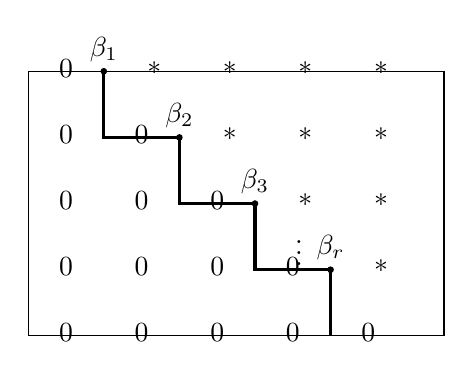
\begin{tikzpicture}[>=latex, scale=0.8]
  \draw (0,0) rectangle (6.6,-4.2);
  \draw[very thick] (1.2,0) -- (1.2,-1.05) -- (2.4,-1.05) -- (2.4,-2.1) -- (3.6,-2.1) -- (3.6,-3.15) -- (4.8,-3.15) -- (4.8,-4.2);
  \fill (1.2,0) circle (1.5pt) node[above]{$\beta_1$};
  \fill (2.4,-1.05) circle (1.5pt) node[above]{$\beta_2$};
  \fill (3.6,-2.1) circle (1.5pt) node[above]{$\beta_3$};
  \fill (4.8,-3.15) circle (1.5pt) node[above]{$\beta_r$};
  \node at (4.3,-2.75) {$\vdots$};
  \node at (0.6,0.05) {$0$};
  \node at (0.6,-1.0) {$0$};
  \node at (1.8,-1.0) {$0$};
  \node at (0.6,-2.05) {$0$};
  \node at (1.8,-2.05) {$0$};
  \node at (3.0,-2.05) {$0$};
  \node at (0.6,-3.1) {$0$};
  \node at (1.8,-3.1) {$0$};
  \node at (3.0,-3.1) {$0$};
  \node at (4.2,-3.1) {$0$};
  \node at (0.6,-4.15) {$0$};
  \node at (1.8,-4.15) {$0$};
  \node at (3.0,-4.15) {$0$};
  \node at (4.2,-4.15) {$0$};
  \node at (5.4,-4.15) {$0$};
  \node at (2.0,0.05) {$*$};
  \node at (3.2,0.05) {$*$};
  \node at (4.4,0.05) {$*$};
  \node at (5.6,0.05) {$*$};
  \node at (3.2,-1.0) {$*$};
  \node at (4.4,-1.0) {$*$};
  \node at (5.6,-1.0) {$*$};
  \node at (4.4,-2.05) {$*$};
  \node at (5.6,-2.05) {$*$};
  \node at (5.6,-3.1) {$*$};
\end{tikzpicture}
\end{center}
的矩阵, 其中在位置 $(1, j_1), \ldots, (r, j_r)$ 处有系数 $\beta_1, \ldots, \beta_r \in K^*$, 且 $j_1 < \cdots < j_r$.则 $B$ 的前 $r$ 行构成由 $A$ 的行向量在 $K^n$ 中生成的线性子空间的一个基.特别地有
\[
\operatorname{rg}_z A = \operatorname{rg}_z B = r\text{.}
\]
\end{bigtheorem}

\begin{proof}
设 $b_1, \ldots, b_m$ 是上面矩阵 $B$ 的行.我们首先证明 $b_1, \ldots, b_r$ 线性无关, 从而构成线性子空间
\[
\langle b_1, \ldots, b_r \rangle = \langle b_1, \ldots, b_m \rangle \subset K^n
\]
的一个基.如果我们能把 $A$ 借助初等行变换化为 $B$(这我们将在下面证明), 那么由定理~\mtref{thm:3.2.3}, 这个子空间恰是由 $A$ 的行向量在 $K^n$ 中生成的线性子空间.特别得到 $\operatorname{rg}_z A = \operatorname{rg}_z B = r$.

例如设 $\sum_{i = 1}^{r}\alpha_i b_i = 0$, 其中 $\alpha_i \in K$ 为某些系数.若记 $B = (\beta_{ij})_{i, j}$, 即 $\beta_{i, j_i} = \beta_i$ ($i = 1, \ldots, r$), 则得到方程组

\[
\begin{array}{r c l r c l r c l r c l}
\alpha_1\beta_1 & & & & & & & & & & & = 0, \\
\alpha_1\beta_{1, j_2} & + & \alpha_2\beta_2 & & & & & & & & & = 0, \\
\alpha_1\beta_{1, j_3} & + & \alpha_2\beta_{2, j_3} & + & \alpha_3\beta_3 & & & & & & & = 0, \\
& & \vdots & & & & & & & & & \\
\alpha_1\beta_{1, j_r} & + & \alpha_2\beta_{2, j_r} & + & \cdots & + & \alpha_r\beta_r & & & & & = 0,
\end{array}
\]

由它先得 $\alpha_1 = 0$, 然后 $\alpha_2 = 0$, 如此继续, 直到最终 $\alpha_r = 0$.于是 $b_1, \ldots, b_r$ 线性无关.

还剩下要证明: 每个矩阵 $A = (\alpha_{ij})_{i, j} \in K^{m \times n}$ 都能化为行阶梯形.为此按如下步骤进行.由于零矩阵已经是行阶梯形, 可以假设 $A \neq 0$.选取最小的指标 $j = j_1$, 使得存在 $i$ 满足 $\alpha_{ij} \neq 0$, 交换第一行与第 $i$ 行, 并令 $\beta_1 = \alpha_{i, j_1}$.通过 $m - 1$ 个保持第一行不变的类型 III 的变换, 可以使 $j_1$ 列中位于 $\beta_1$ 下方的所有元素都变为零.所得矩阵具有如下形状:

\[
\begin{pmatrix}
0 & \cdots & 0 & \beta_1 & * & \cdots & * \\
\hline
0 & \cdots & 0 & 0 & & \\
\vdots & & \vdots & \vdots & & A^{(1)} \\
0 & \cdots & 0 & 0 & &
\end{pmatrix}
\]

现在可以第二步把同一方法应用于 $A^{(1)}$ 以代替 $A$.把对 $A^{(1)}$ 所需的变换解释为整个矩阵的行变换, 并足够多次地重复这一方法, 就可用递归方式实现所断言的行阶梯形.若在某一步首次把 $A^{(r)}$ 化为零矩阵或空矩阵, 则构造终止.
\end{proof}

我们来看一个把矩阵化为行阶梯形的例子:

\[
\begin{pmatrix} 0 & 0 & 2 \\ 0 & 2 & 4 \\ 0 & 1 & 1 \end{pmatrix}
\longmapsto
\begin{pmatrix} 0 & 1 & 1 \\ 0 & 2 & 4 \\ 0 & 0 & 2 \end{pmatrix}
\longmapsto
\begin{pmatrix} 0 & 1 & 1 \\ 0 & 0 & 2 \\ 0 & 0 & 2 \end{pmatrix}
\longmapsto
\begin{pmatrix} 0 & 1 & 1 \\ 0 & 0 & 2 \\ 0 & 0 & 0 \end{pmatrix}
\]

高斯消元法尤其可以用来计算由给定向量生成的线性子空间 $U = \langle a_1, \ldots, a_m \rangle \subset K^n$ 的维数, 或给出 $U$ 的一个基.结合维数公式~\mtref{thm:1.6.5}, 还可以确定两个线性子空间 $U, U' \subset K^n$ 的交 $U \cap U'$ 的维数.进一步, 对线性映射 $f \colon K^n \longrightarrow K^m$, 自然可以确定像的一个基, 从而尤其确定秩 $\operatorname{rg} f$(此时把 $K^m$ 中的向量最好理解为行向量).再由维数公式~\mtref{thm:2.1.10} 还可以得到 $f$ 的核的维数.高斯消元法还适合给出 $\ker f$ 的一个基, 这一点我们将在 \ref{sec:3.5} 节关于线性方程组的部分看得更仔细.在解这些方程组时, 高斯方法导致未知量系统的逐步缩减, 直到最终得到一个其值可自由选取的剩余系统.于是某些未知量被去掉(消去), 所以"消元法"这个名称是说得通的.

与初等行变换相类似, 自然也可以定义矩阵的\emph{初等列变换}(\textup{elementare Spaltenumformungen})\index{chudengliebianhuan@初等列变换(elementare Spaltenumformungen)}.这样的变换可以解释为从右边乘以合适的初等矩阵, 并且像大定理~\mtref{bigthm:3.2.4} 那样可以证明, 每个矩阵都可以化为\emph{列阶梯形}(\textup{Spaltenstufenform})\index{liejietixing@列阶梯形(Spaltenstufenform)}.不过我们不必把所有细节都考虑一遍, 因为接下来我们要处理矩阵的转置.在这个过程下, 初等行变换变为初等列变换, 反之亦然.行阶梯形或列阶梯形的矩阵也如此.

\begin{definition}[\emph{转置矩阵}\index{zhuanzhijuzhen@转置矩阵(transponierte Matrix)}]\label{def:3.2.5}\index{zhuanzhijuzhen@转置矩阵(transponierte Matrix)}
设
\[
A = (\alpha_{ij})_{\substack{i = 1, \ldots, m\\ j = 1, \ldots, n}} \in K^{m \times n}\text{.}
\]
则
\[
A^t = (\alpha_{ij})_{\substack{j = 1, \ldots, n\\ i = 1, \ldots, m}} \in K^{n \times m}
\]
称为 $A$ 的转置矩阵.
\end{definition}

$A^t$ 的行由 $j = 1, \ldots, n$ 参数化, 列由 $i = 1, \ldots, m$ 参数化, 其中 $A^t$ 在位置 $(j, i)$, 即 $j$ 行与 $i$ 列的交点处, 具有系数 $\alpha_{ij}$, 它位于 $A$ 的位置 $(i, j)$ 处.换言之, $A^t$ 由 $A$ 交换行指标与列指标而得到.这相当于 $A$ 关于主对角线(即由位置 $(i, i)$, $i = 1, \ldots, \min(m, n)$ 组成的对角线)的反射.于是 $A$ 的行向量构成 $A^t$ 的列向量, 相应地 $A$ 的列向量构成 $A^t$ 的行向量.直接可见:

\begin{remark}\label{rem:3.2.6}
映射 $K^{m \times n} \longrightarrow K^{n \times m}$, $A \longmapsto A^t$, 是 $K$-向量空间的同构.特别地, 对 $A, B \in K^{m \times n}$, $\alpha \in K$ 有
\[
(A + B)^t = A^t + B^t, \qquad (\alpha A)^t = \alpha A^t\text{.}
\]
\end{remark}

\begin{remark}\label{rem:3.2.7}
对 $A \in K^{m \times n}$ 有
\[
(A^t)^t = A, \qquad \operatorname{rg}_z A = \operatorname{rg}_s A^t, \qquad \operatorname{rg}_s A = \operatorname{rg}_z A^t\text{.}
\]
\end{remark}

\begin{remark}\label{rem:3.2.8}
对可相乘的矩阵 $A, B$ 有
\[
(A \cdot B)^t = B^t \cdot A^t\text{.}
\]
\end{remark}

我们只给出注记~\mtref{rem:3.2.8} 的证明.对

\[
A = (\alpha_{ij})_{i, j} \in K^{m \times n}, \qquad B = (\beta_{jk})_{j, k} \in K^{n \times p}
\]

有

\[
\begin{array}{c}
(A \cdot B)^t = \left(\left(\sum_j \alpha_{ij}\beta_{jk}\right)_{i, k}\right)^t
= \left(\sum_j \alpha_{ij}\beta_{jk}\right)_{k, i} \\
= \left(\sum_j \beta_{jk}\alpha_{ij}\right)_{k, i} = B^t \cdot A^t,
\end{array}
\]

正如所断言的.

下面我们证明, 矩阵的转置对应线性映射的对偶.

\begin{theorem}\label{thm:3.2.9}
设 $f \colon V \longrightarrow W$ 是带 $V$ 的基 $X$ 与 $W$ 的基 $Y$ 的有限维 $K$-向量空间之间的线性映射.若 $X^*$(相应地 $Y^*$)是 $X$(相应地 $Y$)的对偶基, 而 $f^* \colon W^* \longrightarrow V^*$ 是 $f$ 的对偶线性映射, 则
\[
A_{f^*, Y^*, X^*} = (A_{f, X, Y})^t\text{.}
\]
\end{theorem}

\begin{proof}
设
\[
\begin{array}{c c}
X = (x_1, \ldots, x_n), & Y = (y_1, \ldots, y_m), \\
X^* = (x_1^*, \ldots, x_n^*), & Y^* = (y_1^*, \ldots, y_m^*),
\end{array}
\]
于是 $x_j^*(x_\nu) = \delta_{j\nu}$ 且 $y_i^*(y_\mu) = \delta_{i\mu}$.特别地, 对 $\varphi \in V^*$, 它关于基 $X^*$ 的唯一线性组合表示由
\[
\varphi = \sum_{j = 1}^{n}\varphi(x_j)x_j^*
\]
给出.这是定理~\mtref{thm:2.1.7} 的一个推论, 我们在定理~\mtref{thm:2.3.5} 的证明中已经看到.于是属于 $f^*$ 的矩阵可以如下描述:
\[
A_{f^*, Y^*, X^*} = \left(f^*(y_1^*)_{X^*}, \ldots, f^*(y_m^*)_{X^*}\right)
= \left(f^*(y_i^*)(x_j)\right)_{\substack{j = 1, \ldots, n\\ i = 1, \ldots, m}}\text{.}
\]
若 $f$ 的矩阵由
\[
A_{f, X, Y} = (\alpha_{ij})_{\substack{i = 1, \ldots, m\\ j = 1, \ldots, n}}, \qquad
\text{即} \qquad f(x_j) = \sum_{\mu = 1}^{m}\alpha_{\mu j}y_\mu
\]
给出, 则对 $i = 1, \ldots, m$ 得到
\[
\begin{array}{l}
f^*(y_i^*) = \sum_{j = 1}^{n}f^*(y_i^*)(x_j) \cdot x_j^* = \sum_{j = 1}^{n}(y_i^* \circ f)(x_j) \cdot x_j^* \\
\qquad = \sum_{j = 1}^{n}y_i^*\left(f(x_j)\right) \cdot x_j^* = \sum_{j = 1}^{n}y_i^*\left(\sum_{\mu = 1}^{m}\alpha_{\mu j}y_\mu\right) \cdot x_j^* \\
\qquad = \sum_{j = 1}^{n}\alpha_{ij} \cdot x_j^*,
\end{array}
\]
这意味着
\[
A_{f^*, Y^*, X^*} = (\alpha_{ij})_{\substack{j = 1, \ldots, n\\ i = 1, \ldots, m}} = (A_{f, X, Y})^t,
\]
正如所断言的.
\end{proof}

现在利用定理~\mtref{thm:2.3.7}, 即在定理~\mtref{thm:3.2.9} 的情形下映射 $f$ 与 $f^*$ 有相同的秩, 再由注记~\mtref{rem:3.2.2} 与注记~\mtref{rem:3.2.7} 得到

\[
\begin{array}{c}
\operatorname{rg}_s A_{f, X, Y} = \operatorname{rg} f = \operatorname{rg} f^* = \operatorname{rg}_s A_{f^*, Y^*, X^*} \\
= \operatorname{rg}_s (A_{f, X, Y})^t = \operatorname{rg}_z A_{f, X, Y}\text{.}
\end{array}
\]

由于矩阵总可以视为线性映射, 作为定理~\mtref{thm:3.2.9} 的推论得到:

\begin{corollary}\label{cor:3.2.10}
对矩阵 $A \in K^{m \times n}$ 有 $\operatorname{rg}_s A = \operatorname{rg}_z A$, 即列秩与行秩一致.
\end{corollary}

正如已经提到的, 从现在起我们将写 $\operatorname{rg} A$ 来代替 $\operatorname{rg}_s A$ 或 $\operatorname{rg}_z A$, 并把这个数称为矩阵 $A$ 的秩.矩阵的列秩与行秩一致是一个非平凡的结果, 我们在这里借助对偶映射的理论以简单的方式得到了它.但也可以换一种方式推出这个结果, 即利用: 当把矩阵 $A$ 从左边或右边乘以所谓可逆矩阵时, $A$ 的行秩与列秩不改变; 参见 \ref{sec:3.4} 节.

最后, 我们要利用推论~\mtref{cor:3.2.10} 说明, 在大定理~\mtref{bigthm:3.2.4} 中描述的矩阵化为行阶梯形的变换也可以在列向量的意义下解释.这尤其在人们想从给定向量组中选出一个极大线性无关子组时是有利的.

\begin{theorem}\label{thm:3.2.11}
设 $A = (a_1, \ldots, a_n) \in K^{m \times n}$ 是列向量为 $a_1, \ldots, a_n \in K^m$ 的矩阵, 它可以借助初等行变换化为行阶梯形 $B$, 其形状如大定理~\mtref{bigthm:3.2.4} 中所述, 其中对 $i = 1, \ldots, r$, 元素 $\beta_i \in K^*$ 分别位于指标为 $j_i$ 的列, 且 $1 \leq j_1 < \cdots < j_r \leq n$.则向量 $a_{j_1}, \ldots, a_{j_i}$ 线性无关, 并且当 $i \leq r$ 分别取为满足 $j_i \leq j$ 的最大值时, 有
\[
\langle a_1, \ldots, a_j \rangle = \langle a_{j_1}, \ldots, a_{j_i} \rangle, \qquad j = 1, \ldots, n\text{.}
\]
\end{theorem}

\begin{proof}
把矩阵 $A$ 通过删去指标 $j$ 不同于 $j_1, \ldots, j_r$ 的某些列,或删去对某个固定的 $j_0 \in \{1, \ldots, n\}$ 而言指标 $j \geq j_0$ 的所有列而缩小为矩阵 $A'$, 则通过对 $B$ 删去相应的列而缩小为矩阵 $B'$, 得到 $A'$ 的相应行阶梯形.于是
\[
\operatorname{rg}_z B' = \operatorname{rg}_z A' = \operatorname{rg}_s A',
\]
所以由 $A'$ 的列生成的线性子空间的维数恰好等于 $B'$ 的秩.特别地, 用这个论证得到系统 $a_{j_1}, \ldots, a_{j_r} \in K^m$ 的线性无关性, 再由推论~\mtref{cor:1.5.14} (ii) 得到所断言的线性子空间相等.
\end{proof}

\aufgaben

\noindent\textbf{习题 1.} 把矩阵
\[
A = \begin{pmatrix}
1 & 2 & 1 & 2 & 1 & 2 \\
2 & 5 & 4 & 5 & 4 & 5 \\
1 & 4 & 6 & 6 & 6 & 6 \\
2 & 5 & 6 & 9 & 7 & 11
\end{pmatrix} \in \mathbb{R}^{4 \times 6}
\]
化为行阶梯形.

\noindent\textbf{习题 2.} 计算矩阵
\[
A = \begin{pmatrix}
1 & 1 & 3 & 2 \\
1 & 1 & 2 & 3 \\
1 & 1 & 0 & 0
\end{pmatrix} \in K^{3 \times 4}
\]
的行秩, 分别对域 $K = \mathbb{Q}$ 与 $K = \mathbb{F}_5$; 其中 $\mathbb{F}_5$ 是 \ref{sec:1.3} 节习题 3 中含 5 个元素的域.(AT 318)

\noindent\textbf{习题 3.} 检验下列 $\mathbb{R}^5$ 中的向量组是否线性无关:
\[
(5, 4, 3, 2, 1), \quad (1, 2, 3, 4, 5), \quad (2, 2, 2, 2, 1), \quad (1, 0, 0, 1, 1), \quad (1, 0, 1, 0, 1)\text{.}
\]

\noindent\textbf{习题 4.} 设 $U \subset \mathbb{R}^4$ 是由向量
\[
(1, 2, 1, 2), \quad (2, 5, 4, 5), \quad (1, 4, 6, 6), \quad (2, 5, 6, 9), \quad (2, 6, 7, 8), \quad (1, 1, 0, 3)
\]
生成的线性子空间.计算 $\dim U$ 并给出 $U$ 的一个基.

\noindent\textbf{习题 5.} 在 $\mathbb{R}^5$ 中给定下列线性子空间:
\[
U = \left\langle (1, 0, 1, 0, 1), (2, 3, 4, 1, 2), (0, 3, 2, 1, 0) \right\rangle
\]
\[
U' = \left\langle (1, -1, 1, 0, 2), (1, 3, 3, 1, 1), (1, 2, 3, 1, 2) \right\rangle
\]
计算 $\dim U$ 与 $\dim U'$, 并证明 $U \subset U'$.(AT 319)

\noindent\textbf{习题 6.} 在 $\mathbb{R}^6$ 中考察线性子空间
\[
U = \left\langle (1, 1, 1, 0, 1, 1), (2, 3, 4, 0, 2, 1), (0, 3, 2, 1, 1, 1) \right\rangle,
\]
\[
U' = \left\langle (2, 6, 6, 2, 2, 1), (0, 9, 4, 3, 0, 1), (1, 2, 3, 1, 2, 1) \right\rangle,
\]
并计算 $\dim(U \cap U')$.

\noindent\textbf{习题 7.} 考察线性形式
\[
\begin{array}{l l}
f_1 \colon \mathbb{R}^5 \longrightarrow \mathbb{R}, & (\alpha_1, \ldots, \alpha_5) \longmapsto (\alpha_2 + \alpha_3 + \alpha_4 + \alpha_5), \\
f_2 \colon \mathbb{R}^5 \longrightarrow \mathbb{R}, & (\alpha_1, \ldots, \alpha_5) \longmapsto (\alpha_1 + 2\alpha_2 - \alpha_3 - \alpha_4), \\
f_3 \colon \mathbb{R}^5 \longrightarrow \mathbb{R}, & (\alpha_1, \ldots, \alpha_5) \longmapsto (5\alpha_1 + 2\alpha_2 - \alpha_3 + 2\alpha_4 - 2\alpha_5), \\
f_4 \colon \mathbb{R}^5 \longrightarrow \mathbb{R}, & (\alpha_1, \ldots, \alpha_5) \longmapsto (\alpha_1 - \alpha_2 + \alpha_4 - \alpha_5),
\end{array}
\]
并检验它们是否在对偶空间 $(\mathbb{R}^5)^*$ 中构成线性无关组.

\noindent\textbf{习题 8.} 线性形式 $f_1, f_2, f_3, f_4$ 如习题 7 中所给.对 $\mathbb{R}$-线性映射
\[
f \colon \mathbb{R}^5 \longrightarrow \mathbb{R}^4, \quad x \longmapsto \left(f_1(x), f_2(x), f_3(x), f_4(x)\right),
\]
确定 $\dim_\mathbb{R} \ker f$ 与 $\dim_\mathbb{R} \operatorname{im} f$.再给出 $\operatorname{im} f$ 的一个基.

\noindent\textbf{习题 9.} 设 $\mathbb{F}_2$ 是含 2 个元素的域.在 $\mathbb{F}_2$-向量空间 $\mathbb{F}_2^{2000}$ 中, 由
\[
v_i = \begin{cases}
0, & \text{若 } i \text{ 不被 } 4 \text{ 整除}, \\
(1 + \delta_{ij})_{j = 1, \ldots, 2000}, & \text{若 } i \text{ 被 } 4, \text{ 不被 } 8 \text{ 整除}, \\
(1 + \delta_{i - 1, j} + \delta_{i + 1, j})_{j = 1, \ldots, 2000}, & \text{若 } i \text{ 被 } 8 \text{ 整除}
\end{cases}
\]
定义一族向量 $(v_i)_{i = 1, \ldots}$.考察由诸 $v_i$ 生成的线性子空间 $U \subset \mathbb{F}_2^{2000}$, 确定 $\dim_{\mathbb{F}_2} U$ 并给出 $U$ 的一个基.(AT 320)

\section{矩阵环与可逆矩阵}\index{juzhenhuan@矩阵环(Matrizenring)}\index{kenijuzhen@可逆矩阵(invertierbare Matrix)}\index{huan@环(Ring)}\label{sec:3.3}

对 $n \in \mathbb{N}$, 在所有 $(n \times n)$-矩阵的集合 $K^{n \times n}$ 上, 与域的情形相类似, 除加法外还有乘法, 不过对 $n \geq 2$ 它不交换.此时形如

\[
\begin{pmatrix} 1 & 0 \\ 0 & 0 \end{pmatrix} \cdot \begin{pmatrix} 0 & 0 \\ 1 & 0 \end{pmatrix} = 0
\]

的等式表明, 对 $n \geq 2$, $K^{n \times n}$ 中存在非平凡\emph{零因子}(\textup{Nullteiler})\index{lingyinzi@零因子(Nullteiler)}.矩阵 $A \in K^{n \times n}$ 称为零因子, 如果存在非零矩阵 $B \in K^{n \times n}$ 使得 $A \cdot B = 0$ 或 $B \cdot A = 0$.

\begin{definition}[\emph{环}\index{huan@环(Ring)}]\label{def:3.3.1}\index{huan@环(Ring)}
带两个运算 $+$ (加法)与 $\cdot$ (乘法)的集合 $R$ 称为环, 如果下列条件成立:
\begin{enumerate}
\item[(i)] $R$ 关于加法是阿贝尔群.
\item[(ii)] 乘法是结合的, 即对 $a, b, c \in R$ 有
\[
(a \cdot b) \cdot c = a \cdot (b \cdot c)\text{.}
\]
\item[(iii)] 加法与乘法满足分配律, 即对 $a, b, c \in R$ 有
\[
a \cdot (b + c) = a \cdot b + a \cdot c, \qquad (a + b) \cdot c = a \cdot c + b \cdot c\text{.}
\]
\end{enumerate}
关于加法的中性元 $0$ 称为 $R$ 的零元.环 $R$ 称为交换的, 如果乘法是交换的.此外, 元素 $e \in R$ 称为单位元, 如果对一切 $a \in R$ 有 $e \cdot a = a = a \cdot e$; 此时也写 $1$ 来代替 $e$.
\end{definition}

环的单位元(若存在)自然唯一确定.环的最简单例子是\emph{零环}(\textup{Nullring})\index{linghuan@零环(Nullring)} $0$.它只由一个元素 $0$ 组成, 带运算 $0 + 0 = 0$ 与 $0 \cdot 0 = 0$; 于是这里 $0$ 既是零元又是单位元.但我们还要给出一些更有意思的例子.

\begin{enumerate}
\item 整数环 $\mathbb{Z}$ 在通常的加法与乘法下是带单位元的\emph{交换环}(\textup{kommutativer Ring mit Eins})\index{jiaohuanhuan@交换环(kommutativer Ring mit Eins)}.
\item 每个域, 例如 $\mathbb{Q}, \mathbb{R}$ 或 $\mathbb{C}$, 都是带单位元的交换环.
\item 设 $V$ 是 $K$-向量空间, $R = \operatorname{Hom}_K(V, V)$ 是 $V$ 的自同态的 $K$-向量空间.若在 $R$ 中把线性映射的通常加法作为加法,把线性映射的复合作为乘法, 则 $R$ 是一个环, 即所谓 $V$ 的\emph{自同态环}(\textup{Endomorphismenring; End$_K$(V)})\index{zitongtaihuan@自同态环(Endomorphismenring; End$_K$(V))}.这个环记作 $\operatorname{End}_K(V)$.它以零映射 $0 \colon V \longrightarrow V$ 为零元, 以恒等映射 $\mathrm{id} \colon V \longrightarrow V$ 为单位元.可以想到, 对 $\dim_K V \geq 2$, $\operatorname{End}_K(V)$ 不交换.
\item 对 $n \in \mathbb{N}$, $n$ 阶方阵的 $K$-向量空间 $K^{n \times n}$ 在 \ref{sec:3.1} 节引入的矩阵加法与乘法下是一个环.其中 $K^{0 \times 0}$ 是零环, $K^{1 \times 1}$ 是一个环, 我们把它按自然方式与域 $K$ 等同.此外, 对 $n \geq 2$, $K^{n \times n}$ 中的乘法不再交换.矩阵 $E = (\delta_{ij})_{i, j} \in K^{n \times n}$, 常也记作 $1$, 是 $K^{n \times n}$ 中的单位元, 称为 $n$ 阶单位矩阵.正如我们开头看到的, 对 $n \geq 2$, $K^{n \times n}$ 含非平凡零因子.
\end{enumerate}

例 (3) 与 (4) 借助 \ref{sec:3.1} 节的结果可以看出是相关的.更确切地有:

\begin{theorem}\label{thm:3.3.2}
设 $V$ 是 $K$-向量空间, $X = (x_1, \ldots, x_n)$ 是 $V$ 的基.则映射
\[
\varPsi \colon \operatorname{End}_K(V) \longrightarrow K^{n \times n}, \qquad f \longmapsto A_{f, X, X},
\]
是环的同构, 即满足
\[
\varPsi(f + g) = \varPsi(f) + \varPsi(g), \qquad \varPsi(f \circ g) = \varPsi(f) \cdot \varPsi(g)
\]
的双射, 对一切元素 $f, g \in \operatorname{End}_K(V)$ 成立.
\end{theorem}

\begin{proof}
由定理~\mtref{thm:3.1.4}, $\varPsi$ 是与加法相容的双射.与乘法的相容性由定理~\mtref{thm:3.1.9} 推出.
\end{proof}

若 $a$ 是带单位元的环 $R$ 的元素, 则元素 $b \in R$ 称为 $a$ 的逆, 如果 $a \cdot b = 1 = b \cdot a$.$a \in R$ 的逆元素(若存在)总是唯一确定的.事实上, 若两个元素 $b, b' \in R$ 都是 $a$ 的逆, 或更准确地说, $b$ 是 $a$ 的逆而仅成立 $a \cdot b' = 1$(或相应地 $b' \cdot a = 1$), 则
\[
b = b \cdot 1 = b \cdot (a \cdot b') = (b \cdot a) \cdot b' = 1 \cdot b' = b',
\]
或相应地
\[
b = 1 \cdot b = (b' \cdot a) \cdot b = b' \cdot (a \cdot b) = b' \cdot 1 = b'\text{.}
\]
$a$ 的逆元素记作 $a^{-1}$, 此时称 $a$ 可逆或称为单位.在域中, 每个元素 $a \neq 0$ 都是单位.另一方面, 在\emph{矩阵环}(\textup{Matrizenring})\index{juzhenhuan@矩阵环(Matrizenring)} $K^{n \times n}$ 中对 $n \geq 2$ 恒有非平凡零因子, 这样的矩阵不可能是单位.事实上, 若 $A \in K^{n \times n}$ 是单位, 而 $B \in K^{n \times n}$ 是满足 $A \cdot B = 0$ 的矩阵, 则用 $A$ 的\emph{逆矩阵}(\textup{inverse Matrix})\index{nijuzhen@逆矩阵(inverse Matrix)} $A^{-1}$ 必得 $B = A^{-1} \cdot A \cdot B = 0$.

\begin{remark}\label{rem:3.3.3}
在带单位元的环 $R$ 中, 一切单位的集合 $R^*$ 关于乘法构成一个群.
\end{remark}

这个断言直接由环或单位的定义性质得出.

\begin{remark}\label{rem:3.3.4}
设 $V$ 是 $K$-向量空间, $f \in \operatorname{End}_K(V)$.则下列条件等价:
\begin{enumerate}
\item[(i)] 存在元素 $g \in \operatorname{End}_K(V)$ 使得 $f \circ g = \mathrm{id}_V = g \circ f$, 即 $f$ 是 $\operatorname{End}_K(V)$ 中的单位;
\item[(ii)] $f$ 是 $V$ 的自同构.
\end{enumerate}
\end{remark}

\begin{proof}
关系 $f \circ g = \mathrm{id}_V$ 蕴含 $f$ 满射, 相应地 $g \circ f = \mathrm{id}_V$ 蕴含 $f$ 单射.于是由条件 (i) 得 (ii); 反过来, 从 (ii) 也推出 (i), 只要把 $g$ 取为 $f$ 的逆映射.
\end{proof}

自同态环 $\operatorname{End}_K(V)$ 的\emph{单位群}(\textup{Einheitengruppe; R*})\index{danweiqun@单位群(Einheitengruppe; R*)}因此恰好由 $V$ 的一切自同构组成.我们把这个群记作 $\operatorname{Aut}_K(V)$, 称之为 $V$ 的\emph{自同构群}(\textup{Automorphismengruppe; Aut$_K$(V)})\index{zitonggouqun@自同构群(Automorphismengruppe; Aut$_K$(V))}.矩阵环 $K^{n \times n}$ 的单位群记作 $\mathrm{Gl}(n, K)$, 称之为\emph{一般线性群}(\textup{allgemeine lineare Gruppe; Gl(n,K)})\index{yibanxianxingqun@一般线性群(allgemeine lineare Gruppe; Gl(n,K))} (general linear group).$\mathrm{Gl}(n, K)$ 的元素称为可逆(或可逆的, 或正则的, 或非奇异的, 或\emph{非退化}(\textup{nicht ausgeartet})\index{feituihua@非退化(nicht ausgeartet)}的)矩阵.

\begin{theorem}\label{thm:3.3.5}
设 $V$ 是 $K$-向量空间, $X = (x_1, \ldots, x_n)$ 是 $V$ 的基.则定理~\mtref{thm:3.3.2} 中的同构
\[
\varPsi \colon \operatorname{End}_K(V) \xrightarrow{\sim} K^{n \times n}, \qquad f \longmapsto A_{f, X, X},
\]
在相应单位群之间限制为同构
\[
\operatorname{Aut}_K(V) \xrightarrow{\sim} \mathrm{Gl}(n, K),
\]
即限制为尊重各自群结构的双射.
\end{theorem}

\begin{proof}
$\varPsi$ 把恒等映射 $\mathrm{id}_V \in \operatorname{End}_K(V)$ 映到单位矩阵 $E \in K^{n \times n}$, 即把 $\operatorname{End}_K(V)$ 的单位元映到 $K^{n \times n}$ 的单位元.由此直接推出 $\varPsi$ 把单位映到单位.由于逆映射 $\varPsi^{-1}$ 具有相应的性质, 断言得证.
\end{proof}

我们要把定理的内容在稍一般的框架中表述出来.

\begin{theorem}\label{thm:3.3.6}
设 $f \colon V \longrightarrow W$ 是带基 $X = (x_1, \ldots, x_n)$ 与 $Y = (y_1, \ldots, y_n)$ 的向量空间之间的 $K$-线性映射.描述矩阵 $A = A_{f, X, Y}$ 可逆, 当且仅当 $f$ 是同构.
\end{theorem}

\begin{proof}
像注记~\mtref{rem:3.3.4} 的证明那样考虑可知, $f$ 双射, 当且仅当存在 $K$-线性映射 $g \colon W \longrightarrow V$ 使得 $f \circ g = \mathrm{id}_W$ 且 $g \circ f = \mathrm{id}_V$.后者由定理~\mtref{thm:3.1.4} 与定理~\mtref{thm:3.1.9} 等价于存在矩阵 $B \in K^{n \times n}$ 使得 $A_{f, X, Y} \cdot B = 1$ 且 $B \cdot A_{f, X, Y} = 1$.
\end{proof}

\begin{corollary}\label{cor:3.3.7}
对矩阵 $A \in K^{n \times n}$, 下列条件等价:
\begin{enumerate}
\item[(i)] $A$ 可逆;
\item[(ii)] 存在矩阵 $B \in K^{n \times n}$ 使得 $B \cdot A = 1$;
\item[(iii)] 存在矩阵 $B \in K^{n \times n}$ 使得 $A \cdot B = 1$;
\item[(iv)] $\operatorname{rg} A = n$.
\end{enumerate}
\end{corollary}

\begin{proof}
把 $A$ 实现为线性映射, 例如实现为映射
\[
f \colon K^n \longrightarrow K^n, \qquad x \longmapsto A \cdot x\text{.}
\]
则关于 $K^n$ 上的标准基, $A$ 就是属于 $f$ 的矩阵.利用定理~\mtref{thm:3.3.5} 与注记~\mtref{rem:3.2.2}, 只需证明下列条件等价:

(i$'$) $f$ 是自同构;

(ii$'$) 存在 $K$-线性映射 $g \colon K^n \longrightarrow K^n$ 使得 $g \circ f = \mathrm{id}$;

(iii$'$) 存在 $K$-线性映射 $g \colon K^n \longrightarrow K^n$ 使得 $f \circ g = \mathrm{id}$;

(iv$'$) $\operatorname{rg} f = n$.

若 $f$ 是自同构, 则条件 (ii$'$), (iii$'$) 与 (iv$'$) 自然成立.反过来, 若 (ii$'$) 成立, 则 $f$ 单射, 由推论~\mtref{cor:2.1.11} 是自同构.在条件 (iii$'$) 或 (iv$'$) 下, $f$ 满射, 从而同样由推论~\mtref{cor:2.1.11} 是自同构.
\end{proof}

推论~\mtref{cor:3.3.7} 的条件 (iv) 给出了检验矩阵 $A \in K^{n \times n}$ 可逆性的有用判据, 这尤其是因为我们可以借助初等行变换明确地确定矩阵的秩; 参见大定理~\mtref{bigthm:3.2.4}.例如可见, 对 $i, j \in \{1, \ldots, n\}$, $i \neq j$ 与 $\alpha \in K^*$, 初等矩阵

\[
E + (\alpha - 1)E_{ii}, \qquad E + \alpha E_{ij}, \qquad E - E_{ii} - E_{jj} + E_{ij} + E_{ji}
\]

在 $K^{n \times n}$ 中可逆; 这里 $E$ 如 \ref{sec:3.2} 节那样是 $K^{n \times n}$ 中的单位矩阵, 而 $E_{ij} = (\delta_{i\mu}\delta_{j\nu})_{\mu, \nu}$.初等矩阵由单位矩阵 $E$ 经初等行变换得到, 因此与后者有相同的秩, 即 $n$; 参见定理~\mtref{thm:3.2.3}.下面我们还要明确确定上述初等矩阵的逆(它们(顺便说)很容易"猜"出来).

我们可以利用刚才的论证把 \ref{sec:3.2} 节处理的高斯消元法推广到矩阵求逆.例如从矩阵 $A \in K^{n \times n}$ 出发, 按大定理~\mtref{bigthm:3.2.4} 用初等行变换把 $A$ 化为行阶梯形 $B$.现在假设 $A$ 可逆, 则由推论~\mtref{cor:3.3.7} 有 $\operatorname{rg} A = \operatorname{rg} B = n$, 并且在大定理~\mtref{bigthm:3.2.4} 的情形下, 元素 $\beta_1, \ldots, \beta_n$ 恰好位于主对角线上, 即:

\[
B = \begin{pmatrix}
\beta_1 & * & \cdots & * \\
0 & \beta_2 & \cdots & * \\
\vdots & \ddots & \ddots & \vdots \\
0 & \cdots & 0 & \beta_n
\end{pmatrix}\text{.}
\]

通过用 $\beta_i^{-1}$, $i = 1, \ldots, n$ 乘第 $i$ 行, 可以假设所有 $\beta_i$ 都取值为 $1$.然后从其余各行减去第 $n$ 行的倍数, 以这种方式使第 $n$ 列中位于 $\beta_n$ 上方的所有元素都变为零.相应地处理其余各列, 于是得到: 在可逆的情形, $A$ 可借助初等行变换化为单位矩阵 $E$.如 \ref{sec:3.2} 节所见, 每个这样的行变换都可以解释为从左边乘以某个初等矩阵.因此我们找到初等矩阵 $S_1, \ldots, S_r \in K^{n \times n}$ 使得

\[
S_r \cdot \ldots \cdot S_1 \cdot A = E,
\]

从右边乘以 $A^{-1}$ 得到 $A^{-1} = S_r \cdot \ldots \cdot S_1$.把

\[
A^{-1} = S_r \cdot \ldots \cdot S_1 \cdot E
\]

写出来, 我们看到: 把 $A$ 化为单位矩阵 $E$ 的那些初等行变换, 也把 $E$ 本身化为矩阵 $A^{-1}$!

因此矩阵求逆的方法可以描述如下: 用一串初等行变换把 $A$ 化为行阶梯形, 并在每一步也对单位矩阵施行相应的行变换.然后若从行阶梯形读出 $\operatorname{rg} A = n$, 则 $A$ 可逆, 于是继续施行变换, 直到把 $A$ 化为单位矩阵.由单位矩阵经相应变换得到的矩阵就是 $A$ 的逆矩阵 $A^{-1}$.例如用这个方法对 $\alpha \in K$, $i \neq j$ 看出:

\[
\begin{array}{r}
\left(E + (\alpha - 1)E_{ii}\right)^{-1} = E + (\alpha^{-1} - 1)E_{ii}, \\
(E + \alpha E_{ij})^{-1} = E - \alpha E_{ij}, \\
(E - E_{ii} - E_{jj} + E_{ij} + E_{ji})^{-1} = E - E_{ii} - E_{jj} + E_{ij} + E_{ji}\text{.}
\end{array}
\]

作为这个方法的一个副产品, 我们还可以记下:

\begin{theorem}\label{thm:3.3.8}
每个可逆矩阵 $A \in \mathrm{Gl}(n, K)$ 都是类型
\[
\begin{array}{c c}
E + (\alpha - 1)E_{ii}, & \alpha \in K^*, \\
E + E_{ij}, & i \neq j,
\end{array}
\]
($1 \leq i, j \leq n$) 的初等矩阵的乘积.其中 $E \in K^{n \times n}$ 是单位矩阵, $E_{ij} = (\delta_{\mu i}\delta_{\nu j})_{\mu, \nu}$.
\end{theorem}

\begin{proof}
我们刚刚看到, $A$ 可以借助 \ref{sec:3.2} 节中类型 I--IV 的初等行变换化为单位矩阵, 而 $A^{-1}$ 是相应初等矩阵的乘积.但类型 III 的初等行变换, 即对 $\alpha \in K^*$ 与某些指标 $i \neq j$ 把第 $j$ 行的 $\alpha$ 倍加到第 $i$ 行, 也可以解释为类型 I 与 II 的初等行变换的一串: 把第 $j$ 行乘以 $\alpha$, 把它加到第 $i$ 行, 然后又把第 $j$ 行乘以 $\alpha^{-1}$.相应地, 类型 IV 的初等行变换, 即对某些指标 $i \neq j$ 交换第 $i$ 行与第 $j$ 行, 也可以解释为类型 I 与 II 的变换的一串: 把第 $j$ 行加到第 $i$ 行, 把第 $j$ 行乘以 $1$, 把第 $i$ 行加到第 $j$ 行, 最后从第 $i$ 行减去第 $j$ 行.其中最后一步是类型 III 的变换, 因此可以分解为类型 I 与 II 的变换的一串.

把上面的论证应用于 $A^{-1}$ 以代替 $A$, 我们看到 $A$ 正如所断言的是与类型 I 和 II 的初等行变换相对应的初等矩阵的乘积.
\end{proof}

若想明确给出给定矩阵 $A \in \mathrm{Gl}(n, K)$ 的初等矩阵分解, 最好按如下步骤进行: 用初等行变换把 $A$ 化为单位矩阵, 从而得到形如 $A^{-1} = S_r \cdot \ldots \cdot S_1$ 的分解, 其中 $S_1, \ldots, S_r$ 是初等矩阵.取逆给出 $A = S_1^{-1} \cdot \ldots \cdot S_r^{-1}$, 其中如上所述, 各 $S_i^{-1}$ 又都是初等矩阵.若想限于定理~\mtref{thm:3.3.8} 中提到的初等矩阵, 则必要时还要把 $S_i^{-1}$ 进一步分解.

\aufgaben

\noindent\textbf{习题 1.} 设 $X$ 是一个集合, $R$ 是带 $1$ 的环.证明: 一切映射 $X \longrightarrow R$ 的集合 $\operatorname{Abb}(X, R)$ 在 $R$ 值函数的通常加法与乘法下构成一个环.描述这个环的单位群.

\noindent\textbf{习题 2.} 给出一个 $K$-向量空间 $V$, 对它存在非单位 $f, g \in \operatorname{End}_K(V)$ 使得 $f \circ g = \mathrm{id}_V$.

\noindent\textbf{习题 3.} 设 $f \colon U \longrightarrow U$ 是有限维 $K$-向量空间的自同态.则下列条件等价: (AT 321)
\begin{enumerate}
\item[(i)] $\operatorname{rg} f < \dim_K U$;
\item[(ii)] $f$ 是 $\operatorname{End}_K(V)$ 中的左零因子, 即存在 $g \in \operatorname{End}_K(V)$, $g \neq 0$, 使得 $f \circ g = 0$;
\item[(iii)] $f$ 是 $\operatorname{End}(V)$ 中的右零因子, 即存在 $g \in \operatorname{End}_K(V)$, $g \neq 0$, 使得 $g \circ f = 0$.
\end{enumerate}
特别地, $\operatorname{End}_K(V)$ 中的左零因子也是右零因子, 反之亦然.在矩阵环 $K^{n \times n}$ 中相应的结论也成立.

\noindent\textbf{习题 4.} 检验下列矩阵的可逆性, 并在可能时给出逆矩阵:
\[
\begin{pmatrix}
1 & 2 & 3 & 2 & 4 \\
1 & 1 & 2 & 2 & 4 \\
1 & 3 & 4 & 3 & 7 \\
2 & 3 & 5 & 3 & 8 \\
0 & 0 & 1 & 0 & 1
\end{pmatrix},
\quad
\begin{pmatrix}
1 & 1 & 1 & 2 & 0 \\
1 & 0 & 2 & 1 & 0 \\
1 & 1 & 1 & 2 & 1 \\
0 & 1 & 2 & 1 & 0 \\
1 & 1 & 1 & 2 & 0
\end{pmatrix} \in \mathbb{R}^{5 \times 5}
\]

\noindent\textbf{习题 5.} 在可能的情况下, 把下列矩阵写为初等矩阵的乘积:
\[
\begin{pmatrix}
1 & 0 & 0 & 1 \\
1 & 1 & 0 & 3 \\
1 & 1 & 1 & 4 \\
1 & 0 & 1 & 2
\end{pmatrix},
\quad
\begin{pmatrix}
1 & 1 & 1 & 1 \\
0 & 1 & 1 & 1 \\
0 & 0 & 1 & 1 \\
0 & 0 & 0 & 1
\end{pmatrix} \quad \in \mathbb{R}^{4 \times 4}
\]

\noindent\textbf{习题 6.} 对 $A \in \mathrm{Gl}(n, K)$ 证明 $(A^{-1})^t = (A^t)^{-1}$.

\noindent\textbf{习题 7.} 对 $m, r, s \in \mathbb{N} - \{0\}$ 考察矩阵
\[
A \in K^{m \times m}, \qquad B \in K^{m \times s}, \qquad C \in K^{r \times m}, \qquad D \in K^{r \times s},
\]
满足
\[
\operatorname{rg} \begin{pmatrix} A & B \\ C & D \end{pmatrix} = m,
\]
其中 $A$ 可逆.证明 $D = C \cdot A^{-1}B$.(AT 323)

\section{基变换}\index{jibianhuan@基变换(Basiswechsel)}\label{sec:3.4}

我们看到, 向量空间之间的 $K$-线性映射在固定基之后可以用矩阵描述.本节尤其要研究: 当过渡到其他基时, 描述矩阵如何改变.我们以基的一个刻画开始.

\begin{remark}\label{rem:3.4.1}
设 $V$ 是带基 $X = (x_1, \ldots, x_n)$ 的 $K$-向量空间.对带系数 $\alpha_{ij} \in K$ 的 $n$ 个元素 $y_j = \sum_{i = 1}^{n}\alpha_{ij}x_i \in V$, $j = 1, \ldots, n$, 考察矩阵 $A = (\alpha_{ij})_{i, j} \in K^{n \times n}$, 即由 $x_j \longmapsto y_j$ 定义的 $K$-线性映射 $f \colon V \longrightarrow V$ 的矩阵 $A_{f, X, X}$.则下列条件等价:
\begin{enumerate}
\item[(i)] $Y = (y_1, \ldots, y_n)$ 是 $V$ 的基;
\item[(ii)] $\operatorname{rg} A = n$;
\item[(iii)] $A \in \mathrm{Gl}(n, K)$, 即 $A$ 可逆.
\end{enumerate}
\end{remark}

\begin{proof}
若 $Y$ 是 $V$ 的基, 则 $f$ 是同构, 由注记~\mtref{rem:3.2.2} 得 $\operatorname{rg} A = \operatorname{rg} f = \dim_K V = n$.若再有 $\operatorname{rg} A = n$, 则由推论~\mtref{cor:3.3.7} 有 $A \in \mathrm{Gl}(n, K)$.由后一条件又由定理~\mtref{thm:3.3.6} 得 $f$ 是同构, 从而 $Y$ 是基.
\end{proof}

若在注记~\mtref{rem:3.4.1} 的情形下 $Y$ 是 $V$ 的基, 则称 $A = (\alpha_{ij})_{i, j}$ 为\emph{基变换的矩阵}(\textup{Matrix eines Basiswechsels})\index{jibianhuandejuzhen@基变换的矩阵(Matrix eines Basiswechsels)}.这时也可以把 $A$ 解释为恒等映射 $\mathrm{id} \colon V \longrightarrow V$ 关于基 $Y$ 与 $X$ 的矩阵, 即 $A = A_{\mathrm{id}, Y, X}$, 我们为了精确说明基变换的方式将总是这样处理.特别地, 由注记~\mtref{rem:3.4.1} 得到, 在固定 $V$ 的基 $X$ 的情形下, 每个矩阵 $A \in \mathrm{Gl}(n, K)$ 都可以解释为某个合适的基 $Y$ 的形式为 $A_{\mathrm{id}, Y, X}$ 的基变换矩阵.由方程

\[
A_{\mathrm{id}, Y, X} \cdot A_{\mathrm{id}, X, Y} = A_{\mathrm{id}, X, X} = 1,
\]

参见定理~\mtref{thm:3.1.9}, 我们读出:

\begin{remark}\label{rem:3.4.2}
设 $V$ 是带有限基 $X$ 与 $Y$ 的 $K$-向量空间.则基变换矩阵 $A_{\mathrm{id}, Y, X}$ 可逆, 它的逆由基变换矩阵 $A_{\mathrm{id}, X, Y}$ 给出.
\end{remark}

进一步由定理~\mtref{thm:3.1.7} 得到:

\begin{remark}\label{rem:3.4.3}
设 $V$ 是带有限基 $X$ 与 $Y$ 的 $K$-向量空间.对 $a \in V$, 用 $a_X$ 或 $a_Y$ 分别表示 $a$ 关于 $X$ 或 $Y$ 的坐标列向量.则
\[
a_X = A_{\mathrm{id}, Y, X} \cdot a_Y, \qquad a_Y = A_{\mathrm{id}, X, Y} \cdot a_X\text{.}
\]
\end{remark}

接下来要研究线性映射的描述矩阵在基变换下如何变化.

\begin{theorem}\label{thm:3.4.4}
设 $f \colon V \longrightarrow W$ 是有限维 $K$-向量空间之间的 $K$-线性映射.若 $X, X'$ 是 $V$ 的基, $Y, Y'$ 是 $W$ 的基, 则
\[
A_{f, X', Y'} = (A_{\mathrm{id}, Y', Y})^{-1} \cdot A_{f, X, Y} \cdot A_{\mathrm{id}, X', X}\text{.}
\]
\end{theorem}

\begin{proof}
把定理~\mtref{thm:3.1.9} 应用于 $f = \mathrm{id}_W \circ f \circ \mathrm{id}_V$, 得到
\[
A_{f, X', Y'} = A_{\mathrm{id}, Y, Y'} \cdot A_{f, X, Y} \cdot A_{\mathrm{id}, X', X},
\]
其中 $A_{\mathrm{id}, Y, Y'} = (A_{\mathrm{id}, Y', Y})^{-1}$.
\end{proof}

\begin{corollary}\label{cor:3.4.5}
设 $f \colon V \longrightarrow V$ 是带基 $X, X'$ 的有限维 $K$-向量空间 $V$ 的自同态.则
\[
A_{f, X', X'} = (A_{\mathrm{id}, X', X})^{-1} \cdot A_{f, X, X} \cdot A_{\mathrm{id}, X', X}\text{.}
\]
\end{corollary}

现在我们还要给出关于矩阵秩的一些应用.

\begin{theorem}\label{thm:3.4.6}
对矩阵 $S \in \mathrm{Gl}(m, K)$, $A \in K^{m \times n}$ 与 $T \in \mathrm{Gl}(n, K)$ 有
\[
\operatorname{rg}(S \cdot A \cdot T) = \operatorname{rg} A\text{.}
\]
\end{theorem}

\begin{proof}
考察线性映射 $f \colon K^n \longrightarrow K^m$, $a \longmapsto A \cdot a$.若在 $K^n$ 与 $K^m$ 中分别采用标准基, 则 $A$ 就是属于 $f$ 的矩阵.再把 $S^{-1}$ 解释为 $K^m$ 中的基变换矩阵, 把 $T$ 解释为 $K^n$ 中的基变换矩阵, 则由注记~\mtref{rem:3.2.2} 与定理~\mtref{thm:3.4.4} 得
\[
\operatorname{rg}(S \cdot A \cdot T) = \operatorname{rg} f = \operatorname{rg} A\text{.}
\]
\end{proof}

\begin{lemma}\label{lem:3.4.7}
设 $f \colon V \longrightarrow W$ 是向量空间之间的 $K$-线性映射, 其中 $\dim_K V = n$, $\dim_K W = m$.设 $r = \operatorname{rg} f$.则存在 $V$ 的基 $X = (x_1, \ldots, x_n)$ 与 $W$ 的基 $Y = (y_1, \ldots, y_m)$, 使得
\[
A_{f, X, Y} = \begin{pmatrix} E_r & 0 \\ 0 & 0 \end{pmatrix},
\]
其中 $E_r$ 是 $(r \times r)$-单位矩阵, 而 $0$ 各表示合适的(也可能为空)系数全为 $0$ 的区域.
\end{lemma}

\begin{proof}
选取 $\operatorname{im} f$ 的基 $y_1, \ldots, y_r$, 并把它扩充为 $W$ 的基 $Y = (y_1, \ldots, y_m)$.再设 $x_1, \ldots, x_r$ 分别是 $y_1, \ldots, y_r$ 在 $f$ 下的原像.由注记~\mtref{rem:2.1.5} 它们线性无关, 并且如定理~\mtref{thm:2.1.10} 的证明中所证明的, 可以用元素 $x_{r + 1}, \ldots, x_n \in \ker f$ 把它们扩充为 $V$ 的基 $X$.于是
\[
f(x_j) = \begin{cases}
y_j, & \text{对 } j = 1, \ldots, r, \\
0, & \text{对 } j = r + 1, \ldots, n,
\end{cases}
\]
从而 $A_{f, X, Y}$ 具有所求的形式.
\end{proof}

\begin{theorem}\label{thm:3.4.8}
设 $A \in K^{m \times n}$ 且 $\operatorname{rg} A = r$.则存在可逆矩阵 $S \in \mathrm{Gl}(m, K)$ 与 $T \in \mathrm{Gl}(n, K)$ 使得
\[
S \cdot A \cdot T = \begin{pmatrix} E_r & 0 \\ 0 & 0 \end{pmatrix},
\]
其中 $E_r$ 是 $(r \times r)$-单位矩阵, 而 $0$ 各表示合适的(也可能为空)系数全为 $0$ 的区域.
\end{theorem}

\begin{proof}
考察线性映射
\[
f \colon K^n \longrightarrow K^m, \quad a \longmapsto A \cdot a,
\]
它关于 $K^n$ 与 $K^m$ 中的标准基的矩阵由 $A$ 给出.由引理~\mtref{lem:3.4.7} 存在 $K^n$ 的基 $X$ 与 $K^m$ 的基 $Y$, 使得 $A_{f, X, Y}$ 具有所断言的形式.由定理~\mtref{thm:3.4.4} 有 $A_{f, X, Y} = S \cdot A \cdot T$, 其中 $S$ 与 $T$ 是基变换矩阵, 因而是可逆矩阵.
\end{proof}

最后我们还要提示, 如何用本节的论证证明: 对矩阵, 列秩总与行秩一致.我们已经在推论~\mtref{cor:3.2.10} 中借助对偶映射的理论推出了这个结果.设 $A \in K^{m \times n}$.把 $A$ 解释为关于 $V$ 的基 $X$ 与 $W$ 的基 $Y$ 的,属于 $K$-线性映射 $f \colon V \longrightarrow W$ 的矩阵 $A_{f, X, Y}$, 则由注记~\mtref{rem:3.2.2}, $A$ 的列秩为 $\operatorname{rg}_s A = \operatorname{rg} f$.可逆矩阵 $S \in \mathrm{Gl}(m, K)$, $T \in \mathrm{Gl}(n, K)$ 可以看作基变换矩阵, 于是利用定理~\mtref{thm:3.4.4} 得 $\operatorname{rg}_s(S \cdot A \cdot T) = \operatorname{rg} f$.由这个论证得到对任意矩阵 $S \in \mathrm{Gl}(m, K)$, $T \in \mathrm{Gl}(n, K)$ 有
\[
\operatorname{rg}_s(S \cdot A \cdot T) = \operatorname{rg}_s A\text{.}
\]
但这个等式对行秩也是正确的, 因为
\[
\operatorname{rg}_z(S \cdot A \cdot T) = \operatorname{rg}_s(S \cdot A \cdot T)^t = \operatorname{rg}_s(T^t \cdot A^t \cdot S^t) = \operatorname{rg}_s A^t = \operatorname{rg}_z A\text{.}
\]
为此除注记~\mtref{rem:3.2.7} 与注记~\mtref{rem:3.2.8} 外, 只需要 $S^t$(相应地 $T^t$)与 $S \in \mathrm{Gl}(m, K)$(相应地 $T$)一样可逆, 这是直接显然的.现在选取 $S$ 与 $T$ 使 $S \cdot A \cdot T$ 具有定理~\mtref{thm:3.4.8} 给出的简单形状, 则自然有 $\operatorname{rg}_s(S \cdot A \cdot T) = \operatorname{rg}_z(S \cdot A \cdot T)$, 于是得到所求的关系
\[
\operatorname{rg}_s A = \operatorname{rg}_s(S \cdot A \cdot T) = \operatorname{rg}_z(S \cdot A \cdot T) = \operatorname{rg}_z A\text{.}
\]

\aufgaben

\noindent\textbf{习题 1.} 证明下列向量组
\[
\begin{array}{l}
X = \left((1, 1, 1, 2, 0), (1, 0, 2, 1, 0), (1, 1, 1, 2, 1), (1, 1, 2, 1, 0), (0, 1, 1, 2, 0)\right), \\
Y = \left((1, 2, 3, 4, 4), (1, 1, 2, 3, 4), (1, 3, 4, 6, 7), (2, 3, 5, 6, 8), (0, 0, 1, 1, 1)\right)
\end{array}
\]
分别构成 $\mathbb{R}^5$ 的基.基变换矩阵 $A_{\mathrm{id}, X, Y}$ 与 $A_{\mathrm{id}, Y, X}$ 是什么?(AT 324)

\noindent\textbf{习题 2.} 设 $V$ 是维数 $n > 0$ 有限的 $K$-向量空间.描述所有把给定的基 $X$ 除了基向量的次序外仍映到自身的基变换矩阵 $A \in K^{n \times n}$.

\noindent\textbf{习题 3.} 设 $V$ 是维数 $n > 0$ 有限的 $K$-向量空间.对给定的矩阵 $A, B \in K^{n \times n}$ 证明下列条件的等价性:
\begin{enumerate}
\item[(i)] 存在矩阵 $S \in \mathrm{Gl}(n, K)$ 使得 $B = S^{-1}AS$;
\item[(ii)] 存在 $f \in \operatorname{End}_K(V)$ 与 $V$ 的基 $X, Y$, 使得 $A_{f, X, X} = A$ 且 $A_{f, Y, Y} = B$.
\end{enumerate}

\noindent\textbf{习题 4.} 对矩阵 $A, B \in K^{m \times n}$ 写 $A \sim B$, 如果存在 $S \in \mathrm{Gl}(m, K)$ 与 $T \in \mathrm{Gl}(n, K)$ 使得 $B = SAT$.证明关系"$\sim$"是一个等价关系, 描述相应的等价类, 并特别给出其个数.(AT 328)

\noindent\textbf{习题 5.} 设 $V \neq 0$ 是带基 $X, Y$ 的有限维 $K$-向量空间, $V^*$ 是带对偶基 $X^*, Y^*$ 的对偶空间.对基变换矩阵 $A = A_{\mathrm{id}, X, Y}$ 与 $A_{\mathrm{id}, X^*, Y^*}$, 有 $A_{\mathrm{id}, X^*, Y^*} = (A^{-1})^t$.

\section{线性方程组}\index{xianxingfangchengzu@线性方程组(lineares Gleichungssystem)}\label{sec:3.5}

对矩阵 $A = (\alpha_{ij})_{i, j} \in K^{m \times n}$ 与向量 $b = (b_1, \ldots, b_m)^t \in K^m$(我们把它理解为列向量),

\[
\begin{array}{c c c c c}
\alpha_{11}x_1 & + & \cdots & + & \alpha_{1n}x_n = b_1, \\
\alpha_{21}x_1 & + & \cdots & + & \alpha_{2n}x_n = b_2, \\
& & \vdots \\
\alpha_{m1}x_1 & + & \cdots & + & \alpha_{mn}x_n = b_m,
\end{array}
\]

或在矩阵写法下

\[
A \cdot x = b,
\]

称为系数为 $\alpha_{ij} \in K$,未知量为 $x_1, \ldots, x_n$(或 $x = (x_1, \ldots, x_n)^t$)的线性方程组.更准确地说, 这里指的是确定满足方程 $A \cdot x = b$ 的一切 $x \in K^n$ 的问题.在 $b = 0$ 的情形, 方程组称为\emph{齐次的}(\textup{homogen; homogenes Gleichungssystem})\index{qicide@齐次的(homogen; homogenes Gleichungssystem)}, 否则称为\emph{非齐次的}(\textup{inhomogen; inhomogenes Gleichungssystem})\index{feiqicide@非齐次的(inhomogen; inhomogenes Gleichungssystem)}.我们要为线性方程组的\emph{解空间}(\textup{Lösungsraum})\index{jiekongjian@解空间(Lösungsraum)}引入一个专门的记号.

\begin{definition}[解空间]\label{def:3.5.1}\index{jiekongjian@解空间(Lösungsraum)}
对矩阵 $A \in K^{m \times n}$ 与列向量 $b \in K^m$, 我们把集合
\[
M_{A, b} = \left\{x \in K^n;\; A \cdot x = b\right\}
\]
称为线性方程组 $A \cdot x = b$ 的解空间.
\end{definition}

我们可以立即作一个平凡但非常重要的观察, 它给出了此类解空间结构的信息:

\begin{remark}\label{rem:3.5.2}
对系数为 $A \in K^{m \times n}$,$b \in K^m$ 的线性方程组 $A \cdot x = b$, 考察 $K$-线性映射 $f \colon K^n \longrightarrow K^m$, $a \longmapsto A \cdot a$.则
\[
M_{A, b} = f^{-1}(b)\text{.}
\]
因此方程组的解空间是 $K^n$ 的一个仿射子空间; 参见定理~\mtref{thm:2.2.11}.
\end{remark}

对 $b = 0$, 特别有 $M_{A, 0} = \ker f$.此时解空间甚至是 $K^n$ 的线性子空间.

我们首先更仔细地研究齐次线性方程组, 即类型为 $A \cdot x = 0$ 的线性方程组.此时解空间 $M_{A, 0}$ 是 $K^n$ 的线性子空间, 总含有平凡解 $0 \in K^n$, 从而非空.

\begin{theorem}\label{thm:3.5.3}
对 $A \in K^{m \times n}$, 齐次线性方程组 $A \cdot x = 0$ 的解空间 $M_{A, 0}$ 是 $K^n$ 的线性子空间, 且
\[
\dim_K M_{A, 0} = n - \operatorname{rg} A\text{.}
\]
\end{theorem}

\begin{proof}
线性映射 $f \colon K^n \longrightarrow K^m$, $a \longmapsto A \cdot a$, 以 $M_{A, 0}$ 为核, 由维数公式~\mtref{thm:2.1.10} 得 $n = \dim_K(\ker f) + \operatorname{rg} f$, 即 $\dim_K M_{A, 0} = n - \operatorname{rg} A$.
\end{proof}

\begin{lemma}\label{lem:3.5.4}
对 $A \in K^{m \times n}$ 与 $S \in \mathrm{Gl}(m, K)$, 线性方程组 $A \cdot x = 0$ 与 $(S \cdot A) \cdot x = 0$ 有相同的解, 即 $M_{A, 0} = M_{SA, 0}$.
\end{lemma}

\begin{proof}
若 $x \in M_{A, 0}$, 即 $A \cdot x = 0$, 则从左边乘以 $S$ 得 $S \cdot A \cdot x = 0$, 即 $x \in M_{SA, 0}$.反过来, 若 $x \in M_{SA, 0}$, 即 $S \cdot A \cdot x = 0$, 则从左边乘以 $S^{-1}$ 得 $A \cdot x = 0$, 即 $x \in M_{A, 0}$.
\end{proof}

引理~\mtref{lem:3.5.4} 的断言在人们想明确求解具体给定的形如 $A \cdot x = 0$ 的齐次线性方程组时特别有用.因为可以应用高斯消元法, 按大定理~\mtref{bigthm:3.2.4} 用初等行变换把 $A$ 化为行阶梯形.由于这样的变换可以解释为从左边乘以初等矩阵, 即可逆矩阵, 所考察的齐次线性方程组的解空间在此过程中不变.因此可以不失一般性地假设 $A$ 具有行阶梯形.为了使记号清晰, 我们从 $A$ 过渡到另一个行阶梯形矩阵 $A'$, 其中各级台阶位于主对角线上, 即过渡到矩阵

\[
A' = \begin{pmatrix}
\alpha_{11} & \cdots & \cdots & \cdots & \cdots & \alpha_{1n} \\
& \alpha_{22} & \cdots & \cdots & \cdots & \alpha_{2n} \\
& & \ddots \\
& & & \ddots \\
& 0 & & & \alpha_{rr} & \cdots & \alpha_{rn} \\
& & & & 0 & \cdots & 0 \\
& & & & & \ddots \\
& & & & 0 & \cdots & 0
\end{pmatrix},
\]

其中 $\alpha_{11}, \ldots, \alpha_{rr} \in K^*$, $r = \operatorname{rg} A$.这样的行阶梯形可以由一般类型的行阶梯形 $A$ 交换列, 即对 $A$ 的列作某种重新编号而得到.若用 $x'$ 表示未知量 $x = (x_1, \ldots, x_n)$ 相应重新编号后的元组, 则由明确写出线性方程组 $Ax = 0$ 与 $A'x' = 0$ 可见, 两个方程组等价.更准确地说, 由 $A'x' = 0$ 的解恢复 $Ax = 0$ 的解, 只需对 $A'x' = 0$ 的解把先前进行的分量重新编号逆过来.这个过程的详细分析借助所谓\emph{置换矩阵}(\textup{Permutationsmatrix})\index{zhihuanjuzhen@置换矩阵(Permutationsmatrix)}在下面的习题 6 与 7 中进行.

于是我们可以假设矩阵 $A$ 具有上述行阶梯形 $A'$.通过施行进一步的初等行变换, 可以实现 $\alpha_{ii} = 1$ ($i = 1, \ldots, r$), 并且使第 $i$ 列中位于 $\alpha_{ii}$ 上方的所有元素消失.于是可以假设矩阵 $A$ 具有形式

\[
\begin{pmatrix}
1 & & & & \alpha_{1, r + 1} & \cdots & \alpha_{1, n} \\
& 1 & & & \alpha_{2, r + 1} & \cdots & \alpha_{2, n} \\
& & \ddots & & \vdots & \ddots & \vdots \\
& & & 1 & \alpha_{r, r + 1} & \cdots & \alpha_{r, n} \\
0 & \cdots & \cdots & \cdots & \cdots & \cdots & 0 \\
0 & \cdots & \cdots & \cdots & \cdots & \cdots & 0 \\
\vdots & & & & & & \vdots \\
0 & \cdots & \cdots & \cdots & \cdots & \cdots & 0
\end{pmatrix},
\]

其中左上角是 $(r \times r)$-单位矩阵.于是要解下面的方程组:

\[
x_i + \sum_{j = r + 1}^{n}\alpha_{ij}x_j = 0, \qquad i = 1, \ldots, r\text{.}
\]

这是无需花什么力气就能做到的, 因为 $x_{r + 1}, \ldots, x_n \in K$ 的值可以任意给定, 而 $x_1, \ldots, x_r$ 的值由此确定为

\[
x_i = -\sum_{j = r + 1}^{n}\alpha_{ij}x_j, \qquad i = 1, \ldots, r\text{.}
\]

解线性方程组 $A \cdot x = 0$ 的工作因此归结为把 $A$ 化为上面给出的特殊行阶梯形.特别地, 人们由此明白, 为什么这个以高斯命名的过程称为消元法: 由第一个方程得到 $x_1$ 依赖于 $x_{r + 1}, \ldots, x_n$, 由第二个方程得到 $x_2$ 依赖于 $x_{r + 1}, \ldots, x_n$, 如此等等.于是未知量被逐步消去, 直到到达一个其值可自由选取的剩余系统.这表现在: 投影

\[
K^n \longrightarrow K^{n - r}, \qquad (a_1, \ldots, a_n)^t \longmapsto (a_{r + 1}, \ldots, a_n)^t,
\]

诱导一个同构 $M_{A, 0} \xrightarrow{\sim} K^{n - r}$.特别地, 我们再次看出 $\dim_K M_{A, 0} = n - r$, 并且显然, 通过提升 $K^{n - r}$ 的一个基(例如标准基)就得到 $M_{A, 0}$ 的一个基.在上面的记号下, 它由向量

\[
v_j = (-\alpha_{1j}, \ldots, -\alpha_{rj}, \delta_{r + 1, j}, \ldots, \delta_{nj})^t, \qquad j = r + 1, \ldots, n
\]

组成.

因此确定齐次线性方程组 $A \cdot x = 0$ 的解空间 $M_{A, 0}$ 的一个基的步骤如下:

把 $A$ 化为上面描述的特殊行阶梯形.对 $j = r + 1, \ldots, n$, 设 $v_j \in K^n$ 是如下向量: 它指标为 $i = 1, \ldots, r$ 的分量分别为 $A$ 的行阶梯形第 $j$ 列相应分量的相反数, 而指标为 $i = r + 1, \ldots, n$ 的分量恰是 $K^{n - r}$ 的第 $j - r$ 个单位向量的分量.则 $v_{r + 1}, \ldots, v_n$ 构成 $M_{A, 0}$ 的一个基.

原则上, 即使我们在化 $A$ 为行阶梯形时不做列交换,从而不重新编号未知量, 这个法则仍然有效.此时, 就 $A$ 的行阶梯形的列指标以及 $v_j$ 的分量指标而言, 指标 $i = 1, \ldots, r$(相应地 $i = r + 1, \ldots, n$)的作用由行阶梯形"跳跃"(相应地不"跳跃")的那些列指标承担.这里我们指的是那些含有(或不含)在大定理~\mtref{bigthm:3.2.4} 记号意义下位于那里的元素 $\beta_1, \ldots, \beta_r \in K^*$ 之一的列.为了在这种情况下也用公式描述解, 我们以 $A$ 的相应特殊行阶梯形为出发点, 它现在具有形状

\[
\begin{pmatrix}
\underline{1} & * & \ldots & * & 0 & * & \ldots & * & \ldots & * & \ldots & * & 0 & * & \ldots & * \\
0 & 0 & \ldots & 0 & \underline{1} & * & \ldots & * & \ldots & * & \ldots & * & 0 & * & \ldots & * \\
0 & 0 & \ldots & 0 & 0 & 0 & \ldots & 0 & \ldots & \underline{1} & * & \ldots & * \\
\vdots \\
0 & 0 & \ldots & 0 & 0 & 0 & \ldots & 0 & \ldots & 0 & \ldots & 0 & \underline{1} & * & \ldots & * \\
0 & 0 & \ldots & 0 & 0 & 0 & \ldots & 0 & \ldots & 0 & \ldots & 0 & 0 & 0 & \ldots & 0 \\
\vdots
\end{pmatrix},
\]

其中第 $i$ 行的下划线元素 $1$ 位于指标为 $j_i$ 的列, 而 $1 \leq j_1 < \cdots < j_r \leq n$.若 $J'$ 表示行阶梯形"不跳跃"的列指标集合的补, 即 $J' = \{1, \ldots, n\} - \{j_1, \ldots, j_r\}$, 则要解线性方程组

\[
x_{j_i} + \sum_{j' \in J'}\alpha_{ij'}x_{j'} = 0, \qquad i = 1, \ldots, r\text{.}
\]

同样可以任意给定 $x_{j'} \in K$ ($j' \in J'$)的值, 并由此计算 $x_{j_i}$ ($i = 1, \ldots, r$)的值.投影

\[
K^n \longrightarrow K^{n - r}, \qquad (a_1, \ldots, a_n)^t \longmapsto (a_{j'})_{j' \in J'}^t
\]

因此给出一个同构 $M_{A, 0} \overset{\sim}{\longrightarrow} K^{n - r}$, 而通过提升 $K^{n - r}$ 的标准基得到 $M_{A, 0}$ 的一个基, 它由向量

\[
v_{j'} = (\xi_{1j'}, \ldots, \xi_{nj'})^t, \qquad j' \in J',
\]

组成, 其中

\[
\xi_{i'j'} = \begin{cases}
-\alpha_{ij'}, & \text{对 } i' = j_i \text{ 其中 } i \in \{1, \ldots, r\}, \\
\delta_{i'j'}, & \text{对 } i' \in J'\text{.}
\end{cases}
\]

我们来看一个例子.设 $K = \mathbb{R}$, $m = 3$, $n = 4$,

\[
A = \begin{pmatrix} 0 & 0 & 1 & 2 \\ 1 & 2 & 1 & 3 \\ 1 & 2 & 2 & 5 \end{pmatrix}\text{.}
\]

线性方程组 $A \cdot x = 0$ 于是详细写成:

\[
\begin{array}{r}
x_3 + 2x_4 = 0, \\
x_1 + 2x_2 + x_3 + 3x_4 = 0, \\
x_1 + 2x_2 + 2x_3 + 5x_4 = 0\text{.}
\end{array}
\]

现在用初等行变换把 $A$ 化为特殊行阶梯形:

\[
A \longmapsto \begin{pmatrix} 1 & 2 & 1 & 3 \\ 0 & 0 & 1 & 2 \\ 1 & 2 & 2 & 5 \end{pmatrix}
\longmapsto \begin{pmatrix} 1 & 2 & 1 & 3 \\ 0 & 0 & 1 & 2 \\ 0 & 0 & 1 & 2 \end{pmatrix}
\longmapsto \begin{pmatrix} 1 & 2 & 0 & 1 \\ 0 & 0 & 1 & 2 \\ 0 & 0 & 0 & 0 \end{pmatrix},
\]

则这个阶梯形恰好只在列指标 $1$ 与 $3$ 处"跳跃".因此按照上面描述的法则, 我们读出解空间 $M_{A, 0}$ 的基:

\[
v_2 = (-2, 1, 0, 0)^t, \qquad v_4 = (-1, 0, -2, 1)^t\text{.}
\]

如果我们论证得更详细些, 还剩下线性方程组

\[
\begin{array}{c}
x_1 + 2x_2 + x_4 = 0, \\
x_3 + 2x_4 = 0
\end{array}
\]

要解.投影

\[
K^4 \longrightarrow K^2, \qquad (a_1, \ldots, a_4)^t \longmapsto (a_2, a_4)^t
\]

给出同构 $M_{A, 0} \longrightarrow K^2$, 我们把 $K^2$ 的标准基提升为 $M_{A, 0}$ 的基:

\[
\begin{array}{l l}
x_2 = 1, \quad x_4 = 0 & \Longrightarrow \quad x_1 = -2, \quad x_3 = 0, \\
x_2 = 0, \quad x_4 = 1 & \Longrightarrow \quad x_1 = -1, \quad x_3 = -2\text{.}
\end{array}
\]

特别地有 $\dim_K M_{A, 0} = 2$, 并且正如上面已经给出的, 我们看出

\[
M_{A, 0} = \left\langle (-2, 1, 0, 0)^t, (-1, 0, -2, 1)^t \right\rangle\text{.}
\]

下面我们要处理一般情形, 即类型为 $A \cdot x = b$ 的非齐次线性方程组, 其中不显式排除 $b = 0$ 的情形.在下面的叙述中, 用 $(A, b) \in K^{m \times (n + 1)}$ 表示由 $A$ 添加 $b$ 作为第 $(n + 1)$ 列而得到的矩阵.

\begin{theorem}\label{thm:3.5.5}
对 $A \in K^{m \times n}$ 与 $b \in K^m$ 考察线性方程组 $A \cdot x = b$.
\begin{enumerate}
\item[(i)] $A \cdot x = b$ 可解(即至少有一个解), 当且仅当 $\operatorname{rg} A = \operatorname{rg}(A, b)$.
\item[(ii)] $A \cdot x = b$ 普遍可解(即对每个 $b \in K^m$ 至少有一个解), 当且仅当 $\operatorname{rg} A = m$.
\item[(iii)] $A \cdot x = b$ 对一切 $b \in K^m$ 至多有一个解, 当且仅当 $\operatorname{rg} A = n$.
\end{enumerate}
\end{theorem}

\begin{proof}
考察线性映射 $f \colon K^n \longrightarrow K^m$, $a \longmapsto A \cdot a$.对 $A \cdot x = b$ 的解空间有 $M_{A, b} = f^{-1}(b)$; 参见注记~\mtref{rem:3.5.2}.因此 $M_{A, b}$ 非空, 当且仅当 $b$ 属于 $f$ 的像.若 $a_1, \ldots, a_n \in K^m$ 是 $A$ 的列, 则 $\operatorname{im} f = \langle a_1, \ldots, a_n \rangle$, 而 $b \in \operatorname{im} f$ 等价于 $\langle a_1, \ldots, a_n \rangle = \langle a_1, \ldots, a_n, b \rangle$.由于 $\langle a_1, \ldots, a_n \rangle$ 总是 $\langle a_1, \ldots, a_n, b \rangle$ 的线性子空间, 由推论~\mtref{cor:1.5.14} (ii), 只要两个空间的维数一致就可以断言它们相等.而维数正是矩阵 $A$ 与 $(A, b)$ 的秩.于是我们看到, $M_{A, b} \neq \varnothing$ 等价于 $\operatorname{rg} A = \operatorname{rg}(A, b)$, 正如 (i) 所断言的.

由于 $M_{A, b} = f^{-1}(b)$, $A \cdot x = b$ 普遍可解, 当且仅当 $f$ 满射, 即 $\operatorname{im} f = K^m$.后者等价于 $\operatorname{rg} f = m$, 从而等价于 $\operatorname{rg} A = m$, 正如 (ii) 所断言的.

最后, (iii) 中考察的 $A \cdot x = b$ 的唯一\emph{可解性}(\textup{Lösbarkeit})\index{kejiexing@可解性(Lösbarkeit)}等价于 $f$ 的单射性.对 $f$ 利用维数公式~\mtref{thm:2.1.10}, 即
\[
n = \dim_K(\ker f) + \operatorname{rg} f,
\]
可见 $f$ 的单射性等价于 $\operatorname{rg} f = n$, 即 $\operatorname{rg} A = n$.
\end{proof}

若在定理~\mtref{thm:3.5.5} 的情形中 $m = n$, 则条件 (ii) 中的普遍可解性等价于条件 (iii) 中的至多唯一可解性.由推论~\mtref{cor:3.3.7} 因此得到:

\begin{corollary}\label{cor:3.5.6}
对矩阵 $A \in K^{n \times n}$, 下列条件等价:
\begin{enumerate}
\item[(i)] 线性方程组 $A \cdot x = b$ 对 $b \in K^n$ 普遍可解;
\item[(ii)] 线性方程组 $A \cdot x = 0$ 只有平凡解;
\item[(iii)] $A$ 可逆.
\end{enumerate}
\end{corollary}

我们还要更仔细地谈谈非齐次线性方程组解空间的结构.下面的结果再次表明, 这样的解空间是仿射子空间.

\begin{theorem}\label{thm:3.5.7}
对 $A \in K^{m \times n}$ 与 $b \in K^m$, 设 $v_0 \in M_{A, b}$ 是线性方程组 $A \cdot x = b$ 的一个解.则 $M_{A, b} = v_0 + M_{A, 0}$.换言之, 非齐次方程组 $A \cdot x = b$ 的全部解都具有形式 $v_0 + v$, 其中 $v_0$ 是这个方程组的任意一个所谓\emph{特解}(\textup{partikuläre Lösung})\index{tejie@特解(partikuläre Lösung)}, 而 $v$ 遍历相应齐次方程组 $A \cdot x = 0$ 的一切解.
\end{theorem}

\begin{proof}
我们再次考察由 $A$ 给出的线性映射
\[
f \colon K^n \longrightarrow K^m, \qquad x \longmapsto A \cdot x,
\]
其中 $M_{A, b} = f^{-1}(b)$.对 $v_0 \in M_{A, b}$, 由注记~\mtref{rem:2.2.2} 得
\[
M_{A, b} = f^{-1}\left(f(v_0)\right) = v_0 + \ker f = v_0 + M_{A, 0},
\]
正如所断言的.
\end{proof}

现在我们还要说明, 如何借助高斯消元法求解非齐次线性方程组.先是一个有用的观察, 它可以看作引理~\mtref{lem:3.5.4} 的推广:

\begin{lemma}\label{lem:3.5.8}
对 $A \in K^{m \times n}$, $b \in K^m$ 与 $S \in \mathrm{Gl}(m, K)$, 线性方程组 $A \cdot x = b$ 与 $(S \cdot A) \cdot x = Sb$ 有相同的解, 即 $M_{A, b} = M_{SA, Sb}$.
\end{lemma}

\begin{proof}
从左边乘以 $S$ 或 $S^{-1}$, 可见对 $x \in K^n$, $A \cdot x = b$ 等价于 $S \cdot A \cdot x = S \cdot b$.
\end{proof}

因此在解线性方程组 $A \cdot x = b$ 时, 可以用初等行变换改变矩阵 $A$, 只要同时把同样的变换也施于 $b$(把它看作 $(m \times 1)$-矩阵); 因为这样的变换可以解释为从左边乘以初等矩阵, 即可逆矩阵.最简单的做法是把 $A$ 与 $b$ 合并成矩阵 $(A, b)$, 并用初等行变换改变这个矩阵.这样的变换分别作用于各列, 特别分别作用于矩阵 $A$ 与列 $b$, 即对 $S \in \mathrm{Gl}(m, K)$ 有 $S \cdot (A, b) = (SA, Sb)$.

与齐次情形一样, 先把 $(A, b)$ 化为行阶梯形.在对未知量 $x_1, \ldots, x_n$ 作可能的重新编号之后, 可以假设变换后的矩阵具有形状

\[
\begin{pmatrix}
1 & & & & \alpha_{1, r + 1} & \cdots & \alpha_{1, n} & \beta_1 \\
& 1 & & & \alpha_{2, r + 1} & \cdots & \alpha_{2, n} & \beta_2 \\
& & \ddots & & \vdots & \ddots & \vdots & \vdots \\
& & & 1 & \alpha_{r, r + 1} & \cdots & \alpha_{r, n} & \beta_r \\
0 & \cdots & \cdots & \cdots & \cdots & \cdots & 0 & \beta_{r + 1} \\
0 & \cdots & \cdots & \cdots & \cdots & \cdots & 0 & 0 \\
\vdots & & & & & & \vdots & \vdots \\
0 & \cdots & \cdots & \cdots & \cdots & \cdots & 0 & 0
\end{pmatrix},
\]

其中左上角是 $(r \times r)$-单位矩阵, 而 $S$ 表示所需初等矩阵的乘积.与齐次情形一样有 $r = \operatorname{rg} A$, 并且可以看出, 条件 $\operatorname{rg} A = \operatorname{rg}(A, b)$ 即 $\operatorname{rg}(SA) = \operatorname{rg}(SA, Sb)$, 等价于 $\beta_{r + 1} = 0$.于是方程组 $A \cdot x = b$ 可解, 当且仅当在上述行阶梯形中 $\beta_{r + 1} = 0$.若后者成立, 则得到

\[
x_i + \sum_{j = r + 1}^{n}\alpha_{ij}x_j = \beta_i, \qquad i = 1, \ldots, r,
\]

作为变换后的方程组.令 $x_{r + 1}, \ldots, x_n = 0$, 就得到一个特解 $v_0$, 其分量为

\[
\xi_j = \begin{cases}
\beta_j, & \text{对 } j = 1, \ldots, r, \\
0, & \text{对 } j = r + 1, \ldots, n\text{.}
\end{cases}
\]

再按已经演示的方法确定齐次方程组 $A \cdot x = 0$ 的解空间 $M_{A, 0}$, 则由定理~\mtref{thm:3.5.7} 得 $M_{A, b} = v_0 + M_{A, 0}$.总之可以确定, 解 $v_0$ 以及解空间 $M_{A, 0}$ 的基 $v_{r + 1}, \ldots, v_n$ 都可以直接从推导出的原矩阵 $(A, b)$ 的特殊行阶梯形读出.与齐次线性方程组的情形相类似, 即使不允许对未知量重新编号, 而改用行阶梯形"跳跃"处的列指标 $j_1, \ldots, j_r$ 代替指标 $i = 1, \ldots, r$, 上述结论也成立.此时要解方程组

\[
x_{j_i} + \sum_{j' \in J'}\alpha_{ij'}x_{j'} = \beta_i, \qquad i = 1, \ldots, r,
\]

其中 $J' = \{1, \ldots, n\} - \{j_1, \ldots, j_r\}$.在这种情况下, 特解 $v_0 \in M_{A, b}$ 由向量 $v_0 = (\xi_1, \ldots, \xi_n)^t \in K^n$ 给出, 其分量为

\[
\xi_j = \begin{cases}
\beta_i, & \text{对 } j = j_i \text{ 其中 } i \in \{1, \ldots, r\}, \\
0, & \text{其余情形}\text{.}
\end{cases}
\]

作为例子, 对 $K = \mathbb{R}$ 求解方程组 $A \cdot x = b$, 其中

\[
A = \begin{pmatrix} 0 & 0 & 1 & 2 \\ 1 & 2 & 1 & 3 \\ 1 & 2 & 2 & 5 \end{pmatrix}, \qquad
b = \begin{pmatrix} 1 \\ 1 \\ 3 \end{pmatrix}\text{.}
\]

相应齐次方程组的解空间 $M_{A, 0}$ 我们已经确定.先把矩阵 $(A, b)$ 化为特殊行阶梯形:

\[
(A, b) \longmapsto \begin{pmatrix} 1 & 2 & 1 & 3 & 1 \\ 0 & 0 & 1 & 2 & 1 \\ 1 & 2 & 2 & 5 & 3 \end{pmatrix}
\longmapsto \begin{pmatrix} 1 & 2 & 1 & 3 & 1 \\ 0 & 0 & 1 & 2 & 1 \\ 0 & 0 & 1 & 2 & 2 \end{pmatrix}
\longmapsto \begin{pmatrix} \underline{1} & 2 & 0 & 1 & 0 \\ 0 & 0 & \underline{1} & 2 & 1 \\ 0 & 0 & 0 & 0 & \underline{1} \end{pmatrix},
\]

由此读出 $\operatorname{rg}(A, b) = 3 > 2 = \operatorname{rg} A$.因此方程组 $A \cdot x = b$ 没有解, 即 $M_{A, b} = \varnothing$.

或者我们还要对 $b = (1, 1, 2)^t$ 考察这个方程组.把 $(A, b)$ 化为特殊行阶梯形给出

\[
(A, b) \longmapsto \begin{pmatrix} 1 & 2 & 1 & 3 & 1 \\ 0 & 0 & 1 & 2 & 1 \\ 1 & 2 & 2 & 5 & 2 \end{pmatrix}
\longmapsto \begin{pmatrix} 1 & 2 & 1 & 3 & 1 \\ 0 & 0 & 1 & 2 & 1 \\ 0 & 0 & 1 & 2 & 1 \end{pmatrix}
\longmapsto \begin{pmatrix} \underline{1} & 2 & 0 & 1 & 0 \\ 0 & 0 & \underline{1} & 2 & 1 \\ 0 & 0 & 0 & 0 & 0 \end{pmatrix}\text{.}
\]

此时有 $\operatorname{rg} A = \operatorname{rg}(A, b) = 2$, 并读出 $v_0 = (0, 0, 1, 0)$ 是特解.

在更详细的论证下, 要考察方程组

\[
\begin{array}{c}
x_1 + 2x_2 + x_4 = 0, \\
x_3 + 2x_4 = 1\text{.}
\end{array}
\]

为计算一个特解, 令 $x_2 = x_4 = 0$, 得到 $x_1 = 0$, $x_3 = 1$, 即 $(0, 0, 1, 0)^t \in M_{A, b}$.由于我们已经证明向量 $(-2, 1, 0, 0)^t$ 与 $(-1, 0, -2, 1)^t$ 构成 $M_{A, 0}$ 的基, 于是得到

\[
M_{A, b} = (0, 0, 1, 0)^t + \left\langle (-2, 1, 0, 0)^t, (-1, 0, -2, 1)^t \right\rangle\text{.}
\]

\aufgaben

\noindent\textbf{习题 1.} 对矩阵与向量
\[
A = \begin{pmatrix}
1 & 1 & 1 & 1 & 1 \\
1 & 0 & 1 & 0 & 1 \\
2 & 3 & 4 & 5 & 6 \\
0 & 2 & 2 & 4 & 4
\end{pmatrix} \in \mathbb{R}^{4 \times 5}, \qquad
b = \begin{pmatrix} 1 \\ 1 \\ 1 \\ 1 \end{pmatrix} \in \mathbb{R}^4, \qquad
b' = \begin{pmatrix} 1 \\ 1 \\ 1 \\ -1 \end{pmatrix} \in \mathbb{R}^4
\]
确定一切解:
\begin{enumerate}
\item[(i)] 齐次线性方程组 $A \cdot x = 0$ 的解;
\item[(ii)] 非齐次线性方程组 $A \cdot x = b$ 的解;
\item[(iii)] 非齐次线性方程组 $A \cdot x = b'$ 的解.
\end{enumerate}

\noindent\textbf{习题 2.} 对实矩阵
\[
A = \begin{pmatrix} 1 & 1 & 1 \\ 1 & 2 & 3 \\ 1 & 4 & 9 \\ 1 & 8 & 27 \end{pmatrix}, \quad
B = \begin{pmatrix} 1 & 1 & 1 & 1 \\ 1 & 2 & 3 & 4 \\ 1 & 4 & 9 & 16 \\ 1 & 8 & 27 & 64 \end{pmatrix}, \quad
C = \begin{pmatrix} 1 & 1 & 1 & 1 & 1 \\ 1 & 2 & 3 & 4 & 5 \\ 1 & 4 & 9 & 16 & 25 \\ 1 & 8 & 27 & 64 & 125 \end{pmatrix}
\]
与向量 $b \in \mathbb{R}^4$, 研究线性方程组 $A \cdot x = b$, $B \cdot x = b$ 与 $C \cdot x = b$ 在 $x \in \mathbb{R}^3$, $x \in \mathbb{R}^4$, $x \in \mathbb{R}^5$ 中的普遍或至多唯一可解性.这些方程组特别对 $b = (1, 0, 0, 0)^t$ 可解吗?

\noindent\textbf{习题 3.} 证明: $K^n$ 中每个仿射子空间都是某个系数在 $K$ 中的线性方程组的解空间.

\noindent\textbf{习题 4.} 设 $f \colon V \longrightarrow W$ 是关于合适基 $X$($V$ 的)与 $Y$($W$ 的)由矩阵
\[
A_{f, X, Y} = \begin{pmatrix}
1 & 1 & 2 & 4 & 8 \\
1 & 2 & 1 & 2 & 1 \\
2 & 2 & 2 & 2 & 1 \\
1 & 2 & 2 & 2 & 2
\end{pmatrix} \in \mathbb{R}^{4 \times 5}
\]
给出的 $\mathbb{R}$-线性映射.确定 $\ker f$ 的一个基.(AT 329)

\noindent\textbf{习题 5.} 在 $\mathbb{R}^6$ 中考察线性子空间
\[
\begin{array}{l}
U = \left\langle (1, 1, 1, 0, 1, 1), (2, 3, 4, 0, 2, 1), (0, 3, 2, 1, 1, 1) \right\rangle, \\
U' = \left\langle (2, 6, 6, 2, 2, 1), (0, 9, 4, 3, 0, 1), (1, 2, 3, 1, 2, 1) \right\rangle,
\end{array}
\]
并通过给出一个基来确定 $U \cap U'$.

\noindent\textbf{习题 6.} 设 $A = (a_1, \ldots, a_n) \in K^{m \times n}$ 是列向量为 $a_1, \ldots, a_n \in K^m$ 的矩阵, $b \in K^m$ 是另一个列向量, 而 $S \in \mathrm{Gl}(n, K)$ 是可逆矩阵.对线性方程组 $Ax = b$ 与 $ASy = b$ 的解空间证明 $M_{A, b} = SM_{AS, b}$.(AT 330)

\noindent\textbf{习题 7.} 在习题 6 的情形中, 设 $S$ 特别是一个置换矩阵.这意味着存在指标 $(1, \ldots, n)$ 的一个重新编号(置换)$(\pi_1, \ldots, \pi_n)$, 使得 $S = (e_{\pi_1}, \ldots, e_{\pi_n})$.其中 $e_1, \ldots, e_n \in K^n$ 表示标准单位列向量.证明:
\begin{enumerate}
\item[(i)] $AS = (a_{\pi_1}, \ldots, a_{\pi_n})$;
\item[(ii)] 对列向量 $x = (x_1, \ldots, x_n)^t \in K^n$ 有 $S^t x = (x_{\pi_1}, \ldots, x_{\pi_n})^t$;
\item[(iii)] $S^t S = E$, 其中 $E = (e_1, \ldots, e_n)$ 是单位矩阵, 即 $S^{-1} = S^t$.
\end{enumerate}
现在利用习题 6 中的等式 $M_{A, b} = SM_{AS, b}$, 再次看出: 在解线性方程组 $Ax = b$ 时, 可以对 $A$ 的列与 $x = (x_1, \ldots, x_n)^t$ 的分量重新编号(即把 $A$ 换成 $AS$, 把 $x$ 换成 $y = S^t x$), 只要对得到的解再逆回来即可(把 $ASy = b$ 的解从左边乘以 $S = (S^t)^{-1}$).

\noindent\textbf{习题 8.} 设 $f \colon V \longrightarrow W$ 是(有限维)$K$-向量空间之间的 $K$-线性映射, $f^* \colon W^* \longrightarrow V^*$ 是相应的对偶映射.对 $b \in W$ 证明: "线性方程" $f(x) = b$ 在 $x \in V$ 中可解, 当且仅当对一切 $\varphi \in \ker f^*$ 有 $\varphi(b) = 0$.(AT 330)

\noindent\textbf{习题 9.} 对维数有限的 $n$ 维 $K$-向量空间 $V$ 考察线性形式 $\varphi_1, \ldots, \varphi_m \in V^*$, 并证明:
\begin{enumerate}
\item[(i)] $\dim_K \langle \varphi_1, \ldots, \varphi_m \rangle = \operatorname{rg} f$, 其中 $f \colon V \longrightarrow K^m$ 定义为 $x \longmapsto (\varphi_1(x), \ldots, \varphi_m(x))$;
\item[(ii)] "线性方程组" $\varphi_i(x) = b_i$, $i = 1, \ldots, m$, 恰好在元素 $b_1, \ldots, b_m \in K$ 的任意选取下都有解 $x \in V$, 当且仅当线性形式 $\varphi_1, \ldots, \varphi_m$ 线性无关.
\end{enumerate}

\noindent\textbf{习题 10.} 设 $V$ 是有限维 $K$-向量空间, $\varphi_1, \ldots, \varphi_m \in V^*$ 是线性形式, $b_1, \ldots, b_m \in K$.证明: "线性方程组"
\[
\varphi_i(x) = b_i, \qquad i = 1, \ldots, m,
\]
在 $x \in V$ 中可解, 当且仅当下列条件成立: 若 $\alpha_1, \ldots, \alpha_m \in K$ 是满足
\[
\sum_{i = 1}^{m}\alpha_i\varphi_i = 0
\]
的系数, 则也有 $\sum_{i = 1}^{m}\alpha_i b_i = 0$.

